\documentclass[11pt,a4paper]{report}

%%%%%%%% PACKAGES %%%%%%%%
\usepackage[utf8]{inputenc}
\usepackage{graphicx}
\usepackage{url}
\def\UrlBreaks{\do\/\do-}
\usepackage{breakurl}
\usepackage[numbers,sort]{natbib}


%\usepackage{algpseudocode}
\usepackage{algorithm}
\usepackage{algorithmic,subfigure}
\usepackage{booktabs}
\usepackage{multirow}
\usepackage{epsfig}
\usepackage{amsthm}
\usepackage{amssymb}
\usepackage{amsmath}
\usepackage{amsfonts}
\usepackage{mathrsfs}
\usepackage{color}
\usepackage{multirow}
\usepackage{tabularx,booktabs}
\usepackage{dcolumn}
\newcolumntype{d}[1]{D{.}{.}{#1}}
\usepackage{rotating} % To use "sidewaystable"


\usepackage{comment} % PS
%\usepackage{pdflscape} % if pdflatex used reverses  also in PDF -- PS
\usepackage{lscape} %   PS
\usepackage{pbox} % 3rd paper
\usepackage[breaklinks,pdfpagelabels,plainpages=false]{hyperref} % Hyperref should be the last package called, to prevent problems
\hypersetup{
  colorlinks,
  citecolor=black,
  filecolor=black,
  linkcolor=black,
  urlcolor=black
}
\textwidth16cm
\oddsidemargin0mm
\evensidemargin\oddsidemargin

%%%%%%%%%%%%%%%%%%%%%%%%%%

%%%%%%%%% MACROS %%%%%%%%%
% This LaTeX file contains some macros for the CC license page.
%\input{aux/creativecommons}

% My self defined commands
%\input{aux/commands}

%%The above aux/commands - PS
% default figure
\newcommand{\DefFig}[5][]{% title, % label, file, width, caption
	\begin{figure}[hbt]
        \centering
		\mbox{#1}\\
        \includegraphics[width=#4\hsize]{#3}
        \caption{#5}
        \label{#2}
    \end{figure}
}

\newtheorem{lemma}{Lemma}
\newtheorem{proposition}{Proposition}
\newtheorem{definition}{Definition}
\newtheorem{observation}{Observation}
%\newtheorem{claim}{Claim}
\newtheorem{theorem}{Theorem}
%\newcommand{\proof}[1]{{\em Proof}}
\newtheorem{claim}{Claim}

\newcommand{\Oh}[1]
  {\ensuremath{\mathcal{O}\!\left( {#1} \right)}}
\newcommand{\forward}
  {\ensuremath{\mathsf{forward}}}
\newcommand{\backward}
  {\ensuremath{\mathsf{backward}}}
\newcommand{\lastchar}
  {\ensuremath{\mathsf{lastchar}}}
\newcommand{\shorter}
  {\ensuremath{\mathsf{shorter}}}
\newcommand{\longer}
  {\ensuremath{\mathsf{longer}}}
\newcommand{\maxlen}
  {\ensuremath{\mathsf{maxlen}}}
\newcommand{\rank}
  {\ensuremath{\mathsf{rank}}}
\newcommand{\select}
  {\ensuremath{\mathsf{select}}}
\newcommand{\rsucc}
  {\ensuremath{\mathsf{succ}}}
\newcommand{\nodelabel}
  {\ensuremath{\mathsf{label}}}
\newcommand{\BWT}
	{\ensuremath{\mathsf{BWT}}}
\newcommand{\C}
	{\ensuremath{\mathsf{C}}}
\newcommand{\LF}
	{\ensuremath{\mathsf{LF}}}
\newcommand{\Psiop}
	{\ensuremath{\mathsf{\Psi}}}
\newcommand{\mus}[1]
	{\SI{#1}{\micro\second}}
\newcommand{\elabel}{\ensuremath{\mathsf{label}}}
\newcommand{\EBWT}{\ensuremath{\mathsf{EBWT}}}
\def\ours{\mbox{\rm {\sc Vari}}}
\newcommand{\ignore}[1]{}

\def\child{\textit{outgoing}}
\def\parent{\textit{incoming}}
\def\cdeg{\textit{outdegree}}
\def\pdeg{\textit{indegree}}
\def\cedge{\textit{cedge}}
\def\search{\textit{index}}
\def\last{\textit{last}}
\def\Node{\textit{Node}}
\def\fwd{\textit{fwd}}
\def\bwd{\textit{bwd}}
%\newcommand{\comment}[1]{} % commented -- PS
\newcommand{\Order}{\mathcal{O}}
\newcommand{\order}{o}
%\newcommand{\order}{\mathcal{o}}
\def\polylog{{\mathop{\mathrm{polylog}}\nolimits}}
\def\rank{\textit{rank}}
\def\select{\textit{select}}
\def\access{\textit{access}}
\def\pred{\textit{pred}}
\def\succ{\textit{succ}}

%% end The above aux/commands - PS


%%%%%%%%%%%%%%%%%%%%%%%%%%

%%%%%%%% SETTINGS %%%%%%%%
% The paths to the graphics files:
\graphicspath{{images/}{generated/}}

% Section counting
\setcounter{secnumdepth}{3}
\setcounter{tocdepth}{3}
%%%%%%%%%%%%%%%%%%%%%%%%%%

\def\pyt#1{}
\def\pyt#1{\marginpar{\tiny #1}} % comment this to remove margin comments

\def\vardir{chapters/variable-order-dbg_sections} % Path for the 2nd paper sections
\def\coldir{chapters/colour-dbg_sections} % Path for the 3rd paper sections

%\includeonly{chapters/introduction}

\begin{document}

\title{Succinct de Bruijn Graphs}
\author{Alex Bowe\\
\texttt{alex@nii.ac.jp} \\ \\
Ph.D. Thesis\\ \\
\textbf{Supervisors:} Takeaki Uno, Kunihiko Sadakane\\ \\
School of Multidisciplinary Sciences \\
Department of Informatics \\
National Institute of Informatics \\
Chiyoda-ku, Tokyo, Japan}

\date{\today}

\maketitle

%\begin{abstract}
%



%\begin{abstract}

%In the 20 years since it was introduced to bioinformatics by Idury and Waterman, the {\em de Bruijn graph} has become a mainstay of modern genomics, essential to genome assembly.
%The wide use and importance of de Bruijn graphs has led to a number of succinct representations, which aim to implement the graph in small space, while still supporting fast navigation operations.
  \section{Motivation:}
%  \noindent
  Iqbal et al. (Nature Genetics, 2012) introduced the {\em colored de Bruijn graph}, a variant of the classic de Bruijn graph, which is aimed at ``detecting and genotyping simple and complex genetic variants in an individual or population''.
Because they are intended to be applied to massive population level data, it is essential that the graphs be represented efficiently.
Unfortunately, current succinct de Bruijn graph representations are not directly applicable to the colored de Bruijn graph, which requires additional information to be succinctly encoded as well as support for non-standard traversal operations.
\section{Results:}
Our data structure dramatically reduces the amount of memory required to store and use the colored de Bruijn graph, with some penalty to runtime, allowing it to be applied in much larger and more ambitious sequence projects than was previously possible.
\section{Availability:} https://github.com/cosmo-team/cosmo/tree/VARI
%\end{abstract}
 \\ \\
%\textbf{Keywords:} de Bruijn graphs, succinct data structures, DNA assembly, pan-genomics
%\end{abstract}

%\include{chapters/LicenseDisclaimer}

\setcounter{tocdepth}{1}
\newpage
\tableofcontents
\newpage


\section{Introduction}

In the 20 years since it was introduced to bioinformatics by ~\cite{IW95}, the {\em de Bruijn graph} has become a mainstay of modern genomics, essential to genome assembly~\citep{Compeau11,sequel,ismb2015}. The near ubiquity of de Bruijn graphs has led to a number of succinct representations, which aim to implement the graph in small space, while still supporting fast navigation operations.  Formally, a de Bruijn graph constructed for a set of strings (e.g., sequence reads) has a distinct vertex $v$ for every unique $(k - 1)$-mer (substring of length $k - 1$) present in the strings, and a directed edge $(u, v)$ for every observed $k$-mer in the strings with $(k - 1)$-mer prefix $u$ and $(k - 1)$-mer suffix $v$. A contig corresponds to a non-branching path through this graph. See~\citep{Compeau11} for a more thorough explanation of de Bruijn graphs and their use in assembly. 

\cite{ICTFM12} introduced the {\em colored de Bruijn graph}, a variant of the classical structure, which is aimed at ``detecting and genotyping simple and complex genetic variants in an individual or population.'' The edge structure of the colored de Bruijn graph is the same as the classic structure, but now to each vertex ($(k - 1)$-mer) and edge ($k$-mer)
% FIXME: node coloring (CORTEX) looses information preserved in edge coloring(VARI), should we discuss this?  i.e. two nodes with the same color may or may not have a connecting edge with that color, but if you only color the nodes, you can't tell which is the case
is associated a list of colors corresponding to the samples in which the vertex or edge label exists. More specifically, given a set of $n$ samples, there exists a set $\mathcal{C}$ of $n$ colors $c_1, c_2, .., c_n$ where $c_i$ corresponds to sample $i$ and all $k$-mers and $(k-1)$-mers that are contained in sample $i$ are colored with $c_i$. A {\em bubble} in this graph corresponds to an undirected cycle, and is shown to be indicative of biological variation by \cite{ICTFM12}. 
{\sc Cortex}, the implementation of \cite{ICTFM12}, uses the colored de Bruijn graph to develop a method of assembling multiple genomes simultaneously, without losing track of the individuals from which $(k - 1)$-mers (and $k$-mers) originated. This graph is derived from either multiple reference genomes, multiple samples, or a combination of both.

Variant information of an individual or population can be deduced from structure present in the colored de Bruijn graph and the colors of each $k$-mer.
As implied by \cite{ICTFM12}, the ultimate intended use of colored de Bruijn graphs is to apply it to massive, population-level sequence data that is now abundant due to next generation sequencing technology (NGS) and multiplexing. These technologies have enabled production of sequence data for large populations, which has led to ambitious sequencing initiatives that aim to study genetic variation for agriculturally and bio-medically important species.  These initiatives include the {\em Genome 10K} project that aims to sequence the genomes of 10,000 vertebrate species~\citep{Haussler:2009}, the {\em iK5} project~\citep{Robinson:2011}, the 150 Tomato Genome ReSequencing project~\citep{tomato1,tomato2}, and the 1001 Arabidopsis project, a worldwide initiative to sequence cultivars of {\em Arabidopsis}~\citep{arabidopsis}.  Hence, the succinct colored de Bruijn graph is applicable in the context of these projects, in that it can assist in variation discovery within a species by analyzing all the data in these projects at once. 

In addition to species-specific initiatives, scientific and regulatory agencies are showing increased interest in shotgun metagenomic sequences for public health purposes~\citep{EMBL-EBI-Metagenomics,Miller2013}, specifically monitoring for antimicrobial resistance (AMR)~\cite{baquero_metagenomic_epi, port_2014_metagenomics_AMR_monitoring}.  AMR is considered one of the top public health threats, with fears that the spread of AMR will lead to increased morbitiy and mortality for many bacterial illnesses~\citep{CARB,FAOActionPlan2016}.  AMR occurs when bacteria express genetic elements that render them impervious to antibiotic treatments.  Importantly, these genetic resistance elements can be exchanged between distantly-related bacteria via multiple genetic mechanisms, which makes AMR an inherently population-level phenomenon~\citep{Baquero2013}.   Shotgun metagenomic sequencing allows access to the entire microbial population in a sample (the "metagenome"), which is of immense value for tracking and understanding the evolution of resistance elements within and across diverse bacteria\citep{MacLean2010}.  This metagenomics approach to AMR surveillance has been applied in both human and agricultural settings~\citep{noyes2016resistome,King2016}, generating hundreds of samples with terabytes of sequence data for relatively small studies.  Given the large number of samples and large size of sequence data involved in these whole-genome and metagenomic projects, it is imperative that the colored de Bruijn graph can be stored and traversed in a space- and time-efficient manner.
 
%the {\em Genome 10K} project that aims to sequence the genomes of 10,000 vertebrate species \cite{Haussler:2009}, the {\em iK5} project where the objective is to sequence the genomes of 5,000 arthropods \cite{Robinson:2011}, the 150 Tomato Genome ReSequencing project that aims to identify the sequence diversity within tomato \cite{tomato}, and the 1001 Arabidopsis  Project that is a worldwide initiative to sequence cultivars of Arabidopsis \cite{arabidopsis}. Given the large number of individuals and sequence data involved in these projects it is imperative that the colored de Bruijn graph is able to be stored and traversed in both a memory and time efficient manner.

\paragraph{Our Contribution}  
We develop an efficient data structure for storage and use of the colored de Bruijn graph. Compared to {\sc Cortex}, the implementation of \cite{ICTFM12}, our new data structure dramatically reduces the amount of memory required to store and use the colored de Bruijn graph, with some penalty to runtime. We demonstrate this reduction in memory through a comprehensive set of experiments across the following three datasets: (1)  four plant genomes, (2) 3,765 {\em Escherichia coli} assemblies,
 and (3) 87 sequenced metagenomic samples from commercial beef production facilities.  We show our method, which we refer to as $\ours$ (Finnish for color), has better peak memory usage on all these datasets. Our plant reference genomes dataset required 101 GB of RAM for  {\sc Cortex} to represent while $\ours$ required only 4 GB.  And  our
largest two datasets contain too many $k$-mers and colors for {\sc Cortex}'s data structure to represent in the 512 GB of RAM available on our bioinformatics servers. $\ours$ is a novel generalization of the succinct data structure for classical de Bruijn graphs due to \cite{BOSS12}, which is based on the Burrows-Wheeler transform of the sequence reads, and thus, has independent theoretical importance.

In addition to demonstrating the memory and runtime of $\ours$, we validate its output using the {\em E.coli} reference genome and a simulated variant.
%s 


\paragraph{Related Work} As noted above, maintenance and navigation of the de Bruijn graph is a space and time bottleneck in genome assembly. Space-efficient representations of de Bruijn graphs have thus been heavily researched in recent years. One of the first approaches was introduced by \cite{Simpson:2009} as part of the development of the ABySS assembler.  Their method stores the graph as a distributed hash table and thus requires 336 GB to store the graph corresponding to a set of reads from a human genome ($>$38x depth paired-end reads from Illumina Genome Analyzer II, HapMap: NA18507\footnote{\url{https://www.ncbi.nlm.nih.gov/sra/?term=SRA010896}}). 
 
 \cite{conway} reduced space requirements by using a sparse bitvector  (by \cite{bitvector}) to represent the $k$-mers (the edges), and used rank and select operations (to be described later) to traverse it. As a result, their representation took 32 GB for the same data set.  Minia, by \cite{wabi}, uses a Bloom filter to store edges. They traverse the graph by generating all possible outgoing edges at each node and testing their membership in the Bloom filter. Using this approach, the graph was reduced to 5.7 GB on the same dataset.  Contemporaneously, \cite{BOSS12} developed a different succinct data structure based on the Burrows-Wheeler transform~\citep{BW94} that requires 2.5 GB.  The data structure of \cite{BOSS12} is combined with ideas from IDBA-UD~\citep{idbaud} in a metagenomics assembler called MEGAHIT~\citep{megahit}.  In practice MEGAHIT requires more memory than competing methods  but produces significantly better assemblies.   \cite{paul} implemented the de Bruijn graph using an FM-index and {\em minimizers}.   Their method uses 1.5 GB on the same NA18507 data.  \cite{BFT} released the Bloom Filter Trie, which is another succinct data structure for the colored de Bruiin graph; however, we were unable to compare our method against it since  it only supports the building and loading of a colored de Bruijn graph and does not contain operations to support our experiments.  SplitMEM~\citep{splitmem} is a related algorithm to create a colored de Bruijn graph from a set of suffix trees representing the other genomes. Lastly, Lin et al. \citep{Lin} point out the similarity between the breakpoint graph, which is traditionally viewed as a data structure to detect breakpoints between genome rearrangements, and the colored de Bruijn graph. 
 

\paragraph{Roadmap} In the next section, we describe our succinct colored de Bruijn graph data structure, generalizing the stucture for classic de Bruijn graphs presented by ~\cite{BOSS12}. Section~\ref{sec:results} then elucidates the practical performance of the new data structure, comparing it to {\sc Cortex}. Section~\ref{sec:conclusion} offers some concluding remarks.



\chapter{Succinct de Bruijn Graphs}

\begin{quote}
We propose a new succinct de Bruijn graph representation.  
If the de Bruijn graph of $k$-mers in a DNA sequence of length $N$ has $m$ edges,
it can be represented in $4m + \order(m)$ bits.
This is much smaller than existing ones.
The numbers of outgoing and incoming edges of a node are computed in constant time, and
the outgoing and incoming edge with given label are found in constant time
and $\Order(k)$ time, respectively.
The data structure is constructed in $\Order(Nk \log m/\log\log m)$
time using no additional space.  
\end{quote}

\section{Introduction}
\label{p1-sec:introduction}
Within the last two decades, assembling a genome from enormous 
amount of reads from various DNA sequencers 
has been one of the most challenging and important 
computational problems in molecular biology. 
Though the problem is proved to be NP-hard~\cite{Mye95}, 
many algorithms have been proposed for the problem (see the 
surveys~\cite{KasMor06,MilKor10,Pop09}). 
Most of these algorithms follow a so-called Overlap-Layout-Consensus strategy, 
where an algorithm first finds overlaps between reads, next layouts 
these reads, and finally finds the consensus genome. 
These algorithms can be categorized into two types, due to the graph used in 
the overlap phase. 

Most old-time assembly algorithms (especially for the long Sanger reads) 
first construct a graph called the {\it overlap graph} 
after finding the overlapping pairs of reads, 
where each node represents a read and edges are constructed between nodes 
{\it iff} the corresponding two reads have an overlap of enough 
length~\cite{BatJaf02,HuaYan05,MyeSut00}. 
But this strategy is difficult to apply against the huge data from more recent 
epoch-making next-generation sequencers (NGSs). 
The NGS machines can sequence vast amount of genome data. 
It makes it computationally very hard to compare all the pairs of reads. 
Moreover, most NGSs cannot 
read long DNA fragments ({\it e.g.}, at most 200bp in the case of Illumina HiSeq2000),  
and their read lengths are not long enough to detect overlaps with enough lengths 
between reads. 
To conquer these problems, many recent assembler algorithms utilize a graph 
called the {\it de Bruijn graph} in the overlap 
phase~\cite{Li:2010,MacPrz09,PTW,SahShi12,Simpson:2009,ZerBir08}, 
instead of the overlap graph. 

A de Bruijn graph is a graph where each node represents a $k$-mer
(a substring of length $k$)
that exists in the reads, and an edge exists {\it iff} there is an 
exact overlap of length $k-1$ between the corresponding $k$-mers. 
The de Bruijn graph can be constructed more efficiently than the overlap graph 
in many cases, 
but the overlap phase is still the bottleneck of most assembly algorithms based 
on the de Bruijn graph. 
This is because storing the de Bruijn graph requires huge amount of memory. 
Thus we focus on reducing the memory required for the de Bruijn graph in this paper. 

There have been proposed only two data structures for
reducing the size of memory for the de Bruijn graph.
The succinct data structure proposed by Conway and Bromage~\cite{conway}
is a data structure that straightforwardly
represents the de Bruijn graph by a bit vector.
Its representation should be smaller than a naive ordinary implementation of
the de Bruijn graph, but it still requires $O(m\cdot k)$ memory,
where $k$ is the $k$-mer length and $m$ is the number of edges in the de Bruijn graph,
which means it would be very large when $k$ is large.
The other data structure is by Ye et al.~\cite{YeMa12}, which
stores only a subset of nodes of the de Bruijn graph to save memory,
but it is not actually the de Bruijn graph.

In this paper, we propose a new succinct representation of a de Bruijn graph
which only requires $m(2+\log \sigma)$ bit to store\footnote{The base of logarithm is $2$.}, where
$\sigma$ is the alphabet size ({\it i.e.}, $\sigma = 4$ in the case of DNA).
The size of this representation is not affected by the value of $k$ and is
much smaller than either of the two previous methods.
Moreover we will present the algorithm to construct the data structure on-line.
Our main result is summarized as follows:
\begin{theorem}
The $k$-dimensional de Bruijn graph of $M$ string of total length $N$ on an alphabet of size $\sigma$
can be stored in $m(2+\log \sigma) + \Order((\sigma+M) \log m) + \order(m \log\sigma)$
bits where $m$ is the number of edges in the graph.  
The numbers of outgoing and incoming edges of a node are computed in $\Order(\log\sigma/\log\log m)$ time,
and the outgoing and incoming edge with given label are found in $\Order(\log\sigma/\log\log m)$ time
and $\Order(k\log^2\sigma/\log\log m)$ time, respectively.
The node for a given $k$-mer is found in $\Order(k\log\sigma/\log\log m)$ time.
If $\sigma = \polylog(m)$, the time complexities become $\Order(1)$, $\Order(1)$, $\Order(k\log\sigma)$,
and $\Order(k)$ time, respectively.
\end{theorem}

\begin{theorem}
The $k$-dimensional de Bruijn graph of a string of length $N$
can be constructed in $\Order\left(Nk \cdot \frac{\log m}{\log \log m}
(1+\frac{\log\sigma}{\log\log m})\right)$ time using no additional space.
This representation can be converted to the static one in 
$\Order\left(\frac{m\log m}{\log \log m}
(1+\frac{\log\sigma}{\log\log m})\right)$ time.
\end{theorem}
For DNA sequences ($\sigma=4$), the succinct de Bruijn graph can be constructed in 
$\Order(Nk \log m/\log\log m)$ time and its space becomes $4m + \order(m)$ bits.
This is much smaller than existing ones.
For example, the succinct representation of Conway and Bromage~\cite{conway}
uses 40.8GB for storing a de Bruijn graph with $m = $ 12,292,819,311 edges
and $k = 27$ (28.5 bits per edge).  
On the other hand, if we use an efficient implementation
of {\rank}/{\select} data structures~\cite{bitvector} for our representation,
the estimated size is less than $5$ bits per edge.  
Therefore the above graph is stored in less than 8GB.
\emergencystretch=20pt\par


%%%%%%%%%%%%%%%%%%%%%%%%%%%%%%%%%%%%%%%%%%%%%%%%%%%%%%%%%%%%%%%%%%%%%%%%%%%%%%

\section{Preliminaries}\label{p1-sec:preliminaries}

\subsection{de Bruijn graphs}
In the original definition~\cite{deBruijn46}, the $k$-dimensional de Bruijn graph of $\sigma$ symbols
is a directed graph representing overlaps between strings of symbols defined as follows.
The graph has $\sigma^k$ nodes, consisting of all length-$k$ strings of the symbols.
A node is denoted by $(u_1,\ldots,u_k)$ where $u_1,\ldots,u_k$ are symbols.
For any pair of nodes $u = (u_1,\ldots,u_k)$ and $v = (v_1,\ldots,v_k)$ 
such that 
$u_2 = v_1, u_3 = v_2, \ldots, u_k = v_{k-1}$, the graph has a directed
edge from $u$ to $v$ labeled with $v_k$.
In this paper we call it the complete $k$-dimensional de Bruijn graph
of $\sigma$ symbols.

The de Bruijn graphs considered in this paper are subgraphs of the complete de Bruijn graph.
We define the $k$-dimensional de Bruijn graph of a string $T$ as follows.
The nodes of the graph correspond to all length-$k$ substrings of $T$.  If the string is of length $N$,
the graph has at most $N-k+1$ nodes.  The edges of the graph are defined in the same way as the complete
de Bruijn graph.  For convenience, we add $k$ characters \$ at the head of the string,
and a \$ at the end.

We can also store a set of $M$ strings $T_1,\ldots,T_M$ as follows.
We append a terminator $\$_i$ to the tail of each string $T_i$,
and concatenate all the strings.  Then we add $k$ characters $\$_0$ at the head.
Figure~\ref{p1-fig:debruijn} shows an example.


%dummy node���lj�����


\begin{figure}[bt]
\begin{center}
  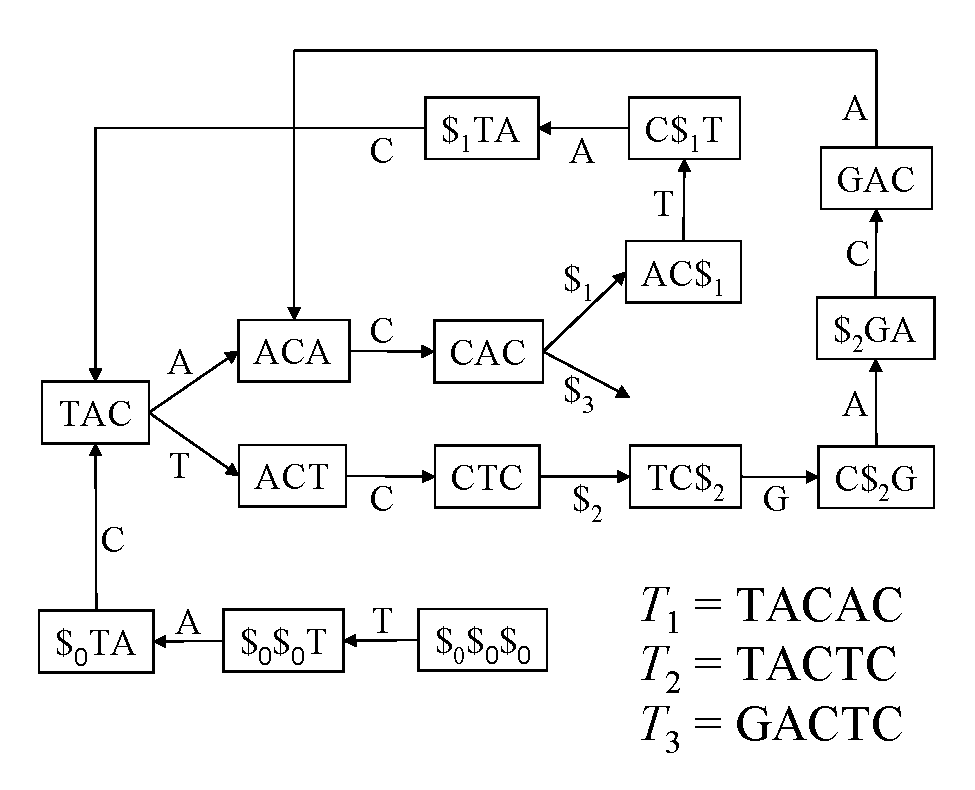
\includegraphics[scale=0.70]{fig3}
\caption{The $3$-dimensional de Bruijn graph of strings `TACAC', `TACTC', and
`GACTC'.}
\label{p1-fig:debruijn}
\end{center}
\end{figure}

\subsection{Basic succinct data structures}\label{p1-sec:rank}

Let $T = T[1] T[2] \cdots T[N]$ be a string of length $N$ on alphabet ${\cal A}$,
that is, $T[i] \in {\cal A}$ for any $i=1,\ldots,N$.
Let $\sigma = |{\cal A}|$ denote the alphabet size.
We can store $T$ in $N \lceil \log_2 \sigma \rceil$ bits.  The space does not
depend on the word size of CPU.  We can retrieve any character $T[i]$ in constant
time using bit operations on words.

The most basic succinct data structure is the one for computing {\rank}, {\select}, and {\access}
values on strings, which are defined as follows.
The value ${\access}(T,i)$ returns $T[i]$ for $1 \le i \le N$.
The value ${\rank}_c(T,i)$ where $c \in {\cal A}$ and $1 \le i \le N$
is the number of $c$'s in $T[1] \cdots T[i]$.  For any $T$ and $c$ we define
${\rank}_c(T,0) = 0$.
The value ${\select}_c(T,j)$ where $c \in {\cal A}$ and $1 \le j \le {\rank}_c(T,N)$
is the position of $j$-th $c$ in $T$.
For any $T$ and $c$ we define ${\select}_c(T,0) = 0$ and for any $j > {\rank}_c(T,N)$
${\select}_c(T,j) = N+1$.
Let $t_r(N,\sigma)$, $t_s(N,\sigma)$, and $t_a(N,\sigma)$ denote the time complexity for computing
{\rank}, {\select}, and {\access}, respectively, on a string of length $N$ and alphabet size $\sigma$.
For brevity, we assume that 
for any $N_1 \le N_2$, $t_r(N_1,\sigma) \le t_r(N_2,\sigma)$ and
for any $\sigma_1 \le \sigma_2$, $t_r(N,\sigma_1) \le t_r(N,\sigma_2)$.
Let $t_b(N,\Sigma)$ denote the maximum of 
$t_r(N,\sigma),t_s(N,\sigma),t_a(N,\sigma)$.

For convenience, we define ${\pred}_c(T,i) = {\select}_c(T, {\rank}_c(T, i))$
which is the position of the first occurrence of $c$ when we scan $T$ from the position $i$ to the head,
and ${\succ}_c(T,i) = {\select}_c(T, {\rank}_c(T, i-1)+1)$
which is the position of the first occurrence of $c$ when we scan $T$ from the position $i$ to the end.
If $T[i]$ is the first (last) occurrence of $c$, {\pred} (\succ) returns $0$ ($N+1$).

%From the definition it holds that
%${\select}_c(T, {\rank}_c(T, i)) \le i$ for any $1 \le i \le n$ and
%${\rank}_c(T, {\select}_c(T, j)) = j$ for any $1 \le j \le {\rank}_c(T,n)$.

There exist many succinct data structures for {\rank} and {\select} on strings.
Among them, we use the one by Ferragina et al.~\cite{FerManMakNav06} for the static case
(the case the string does not change).  A string of $T$ length $n$ on an alphabet of size $\sigma$
can be stored in $nH_0(T) + \Order(\sigma \log n) + \order(n \log\sigma)$ bits so that
{\rank}, {\select} and {\access} queries take $\Order(\log\sigma / \log\log n)$ time,
where $H_0(T)$ denotes the order-$0$ entropy of the string.  Note that if the alphabet size $\sigma$
is $\polylog(n)$, the queries are done in constant time.  For a binary alphabet case,
we can use a simpler data structure that has the same time and space complexities~\cite{RRR07}.

For the dynamic case where the string is modified by inserting or deleting a character,
we use the one by Navarro and Sadakane~\cite{NavSad10} which stores the string
in $nH_0(T) + \Order(\sigma \log n) + \order(n \log\sigma)$ bits so that
{\rank}, {\select} and {\access} queries and insertion and deletion of a character take
$\Order(\frac{\log n}{\log \log n}(1+\frac{\log\sigma}{\log\log n}))$ time.
For polylog-sized alphabets, the operations are done in optimal $\Order(\log n/\log \log n)$ time.
The time complexities for insert and delete are denoted by $t_u(n,\sigma)$.


\subsection{The XBW data structure}
The XBW-transform~\cite{FLMM09} is a method for compressing and indexing labeled trees.
It is an extension of the Burrows-Wheeler transform~\cite{BW94} used for compressing
and indexing strings.  Given a rooted tree with $n$ nodes where each node has a label in
the set of size $\sigma$, the XBW-transform converts the tree into a representation of
$2n + n \log\sigma$ bits.  The size of the representation matches the information-theoretic
lower bound.  We can support tree navigational operations by adding small-size auxiliary
indexes.

Because the XBW is for storing a tree, we cannot use it directly for storing de Bruijn graphs,
which is a cyclic graph.
This paper proposes a new compact representation of de Bruijn graphs of strings.


%%%%%%%%%%%%%%%%%%%%%%%%%%%%%%%%%%%%%%%%%%%%%%%%%%%%%%%%%%%%%%%%%%%%%%%%%%%%%%

\section{Succinct de Bruijn Graphs}\label{p1-sec:sdg}

Let $G$ be a $k$-dimensional de Bruijn graph of a string $T$ of length $N$ on alphabet ${\cal A}$.
Let $n$ and $m$ be the numbers of nodes and edges of $G$, respectively.
A succinct representation of $G$ supports the following operations:
\begin{itemize}
\item ${\cdeg}(v)$ returns the number of outgoing edges from node $v$.
%\item ${\cedge}(v, i)$ 
%\item ${\child}(v, i)$ returns the node $w$ pointed to by the $i$-th outgoing edge of node $v$
%($1 \le i \le {\cdeg}(v)$).
\item ${\child}(v, c)$ returns the node $w$ pointed to by the outgoing edge of node $v$
with edge label $c$.  If no such node exists, it returns $-1$.
\item ${\pdeg}(v)$ returns the number of incoming edges to node $v$.
%\item ${\parent}(v, i)$ returns the node $w$ that is on the $i$-th incoming edge of node $v$
%($1 \le i \le {\pdeg}(v)$).
\item ${\parent}(v, c)$ returns the node $w = (w_1,\ldots,w_k)$ such that 
there is an edge from $w$ and $v$
and $w_1 = c$.  If no such node exists, it returns $-1$.
\item ${\search}(s)$ returns the index $i$ of the node whose label is the string $s$ of length $k$.
%Precisely, $i$ such that ${\last}[i] = 1$ and ${\Node}[i] = s$.
\end{itemize}

We define ${\cal A}^-$ as any set of size $|{\cal A}|$ such that ${\cal A}^- \cap {\cal A} = \emptyset$.
Let $c^-$ denote an element of ${\cal A}^-$ corresponding to an element $c \in {\cal A}$.
We also define a function $u$ as $u(c^-) = c$ for any $c^- \in {\cal A}^-$
and $u(c) = c$ for any $c \in {\cal A}$.  We assume that the function is evaluated in constant time.

\subsection{The succinct representation}

The representation consists of the following components:
\begin{itemize}
\item a string $W = W[1] W[2] \cdots W[m]$ where each character is from ${\cal A} \cup {\cal A}^-$.
\item a string ${\last}$ of length $m$ on the binary alphabet $\{0,1\}$.
\item an array $F$ of length $\sigma = |{\cal A}|$.
\end{itemize}
An example is shown in Figure~\ref{p1-fig:succinctdebruijn}.

The string $W$ is defined as follows.
Each character $W[i]$ represents the label of an edge of $G$.
Each edge $u \rightarrow v$ of $G$ is associated with the node label of $u$.
Those edge labels are sorted in the lexicographic order of reversals of associated node labels.
Ties are broken by edge labels.
Let ${\Node}[i]$ denote the node label for $W[i]$.  This is not explicitly stored.

The string ${\last}$ is defined as
${\last}[i] = 1$ if $i = n$ or ${\Node}[i]$ is different from ${\Node}[i+1]$,
or ${\last}[i] = 0$ otherwise.  From this definition,
all node labels ${\Node}[i]$ with ${\last}[i] = 1$ are distinct, and
those indices $i$ have one-to-one correspondence with the nodes of $G$.
Therefore we use an index $i$ of the strings such that ${\last}[i] = 1$
to represent a node $v$.  
%There are $n$ such indices.
Let $n$ denote the number of nodes.

The array $F$ stores cumulative frequencies of the last characters of node labels.
Namely, for any $c \in {\cal A}$, 
%$F[c] = |\{i \mid 1 \le i \le m, \mbox{the last character of ${\Node}[i]$ is
%smaller than $c$}  \}|$
$F[c] = |\{i \mid 1 \le i \le m, C(i) < c  \}|$
where $C(i)$ denotes the last character of ${\Node}[i]$.
Because $F[\$_i] = i$ for $i = 0,1,\ldots,M$, we need not store them.

The array $F$ is represented in $\Order(\sigma \log m)$ bits.
If $F$ does not change, we can store it as it is using a simple array and $F[c]$ is computed
in constant time.
In a dynamic case that a new node or edge is inserted to the de Bruijn graph,
we have to update $F$ accordingly.  By using a balanced binary tree, $F$ can be maintained
in $\Order(\log \sigma)$ time.

We also use the inverse of $F$, that is, given $i$, we need to know the last character $c$
of ${\Node}[i]$.  In a static case, this can be
computed in constant time using a {\rank}/{\select} data structure of
$\Order(\sigma \log m) + \Order(m \log\log m/\log m)$ bits~\cite{RRR07}.
In a dynamic case, it is done in $\Order(\log \sigma)$ time using a balanced
binary search tree.
%
It can be improved to $\Order(\frac{\log m }{\log \log m}
(1+\frac{\log\sigma}{\log\log m}))$ time using \cite{NavSad10}.
This data structure uses
$\Order(\sigma \log n) + \Order(m \log \log m/\log m)$ bits.
%
Let $t_f$ denote the largest time complexity of those operations.


\begin{figure}[bt]
\begin{center}
  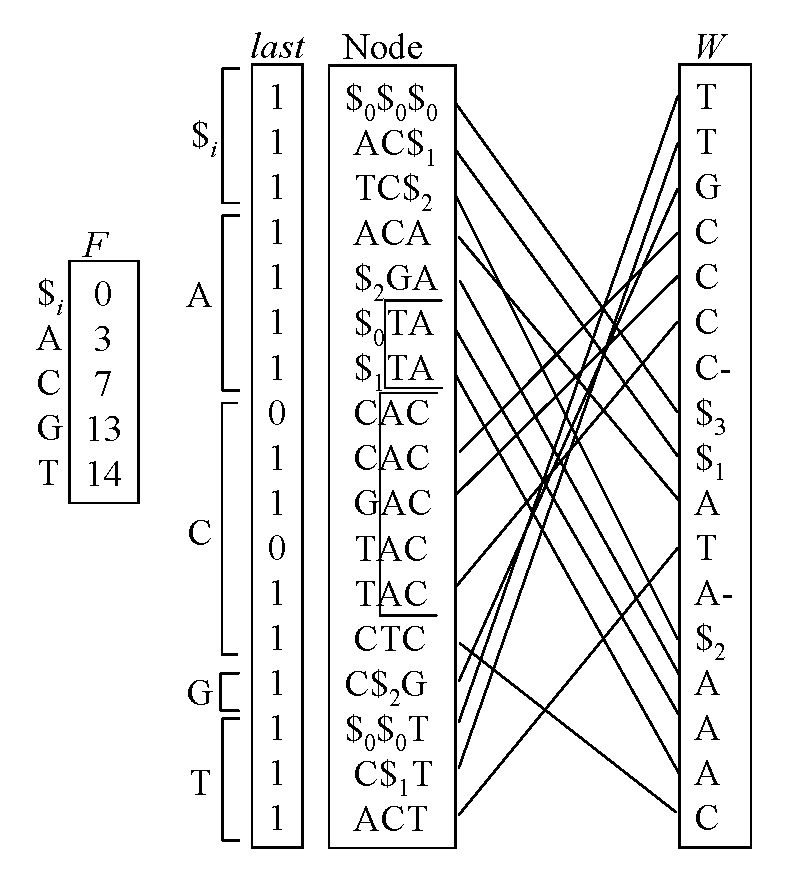
\includegraphics[scale=0.70]{fig4}
\caption{The succinct representation of the de Bruijn graph in Figure~\ref{p1-fig:debruijn}.
Lines between {\Node} and $W$ show {\fwd} and {\bwd} functions.
}
\label{p1-fig:succinctdebruijn}
\end{center}
\end{figure}


A character $W[i]$ is from either ${\cal A}$ or ${\cal A}^-$.
If $W[i]$ is from ${\cal A}^-$, it means that there exists $j < i$ such that
$W[j] = u(W[i])$ and ${\Node}[j]$ and ${\Node}[i]$ have the identical suffix of length $k-1$.

We can define a one-to-one mapping between indices $i$ of ${\last}$ with ${\last}[i] = 1$
and indices $j$ of $W$ with $W[j] \in {\cal A}$.
As stated above, the indices $i$ with ${\last}[i] = 1$ have one-to-one correspondence with
the nodes of the de Bruijn graph $G$.  Consider indices $j$ with $W[j] \in {\cal A}$.
Let ${\Node}^\prime[j]$ denote
the concatenation of the length $k-1$ suffix of ${\Node}[j]$ and $W[j]$.
For any ${\Node}^\prime[j]$, there exists $i$ such that ${\Node}[i] = {\Node}^\prime[j]$.
Because of the definition of $W$, there are no indices $j$ and $j^\prime$ 
($j \neq j^\prime$) such that ${\Node}^\prime[j] = {\Node}^\prime[j^\prime]$.
Therefore there is a one-to-one mapping.  Furthermore, the mapping is represented by
{\rank} and {\select} queries on $W$.
Let $i,j$ be indices such that ${\last}[i] = 1$ and ${\Node}[i] = {\Node}^\prime[j]$.
Let $c = C(i)$ be the last character of ${\Node}[i]$ and 
$r = {\rank}_1({\last}, i) - {\rank}_1({\last}, F[c])$.
Then it holds $j = {\select}_c(W, r)$.  
From $j$, $i$ is computed by $c = W[i]$, $r = {\rank}_c(W, j)$ and
$i = {\select}_1({\last}, {\rank}_1({\last}, F[c]) + r)$.
We define $\bwd(i) = j$ and $\fwd(j) = i$.
The time complexities of $\bwd(i)$ and $\fwd(j)$ are
$\Order(t_f + t_b(m,2\sigma))$.

%Note that the function ${\bwd}(i^\prime)$ for ${\last}[i^\prime] = 0$
%returns the same value as ${\bwd}(i)$ where $i$ is the index such that
%${\last}[i] = 1$ and ${\Node}[i^\prime] = {\Node}[i]$.

Our data structure is similar to the XBW data structure~\cite{FLMM09} in the sense
that the {\last} array in ours is the same as $S_{\last}$ in the XBW.
We propose a new encoding scheme for storing labels of a graph.


\subsection{The {\cdeg} and {\child} operations}
The ${\cdeg}(v)$ operation is easy to support.
We assume that $v$ is the index of ${\last}$ such that ${\last}[v] = 1$ and
${\Node}[v]$ is the label of the node.
From the definition of ${\last}$, it is obvious that 
${\cdeg}(v) = v - {\pred}_1({\last}, v-1)$.
The time complexity is $\Order(t_b(m,2))$.

The ${\child}(v,c)$ operation is done as follows.
For any $1 \le i \le m$, we define $R(i) = [{\pred}_1({\last},i-1)+1,{\succ}_1({\last},i)]$,
which is the range of $W$ and ${\last}$ that for all $j \in R(i)$, ${\Node}[j]$ are identical.
The labels of outgoing edges of node $v$ are stored in $W[j]$ for $j \in R(v)$.
%and they are sorted.  
%
%binary search�����Ȃ��Ă��Crank/select�ł����Ȃ苁�܂��D
%We perform a binary search in the range using the ${\access}$ operation
%on $W$.  Note that during the binary search we regard any character $a^- \in {\cal A}^-$
%as the corresponding character $a$ in ${\cal A}$.
Let $j$ be the index such that $u(W[j]) = c$.
We can find $j$ by ${\pred}_c(W, v)$ and ${\pred}_{c^-}(W, v)$.
Then $x = {\child}(v,c)$ can be computed by $x = \fwd(j)$.

The time complexity for ${\child}(v,c)$ is 
$\Order(t_f + t_b(m, 2\sigma))$.

\subsection{The {\pdeg} and {\parent} operations}
Consider to compute ${\pdeg}(v)$.
Let $d = C(v)$ and $x = bwd(v)$.  Then it holds $d = W[x]$ and the first character
of ${\Node}[x]$ is the label of an edge pointing to $v$.
Let $y = {\succ}_d(W, x)$.  Then all $d^-$ between $W[x]$ and $W[y]$ correspond
to parents of $v$.  The number of such $d^-$ is computed by {\rank} on $W$.
The time complexity is $\Order(t_f + t_b(m,2\sigma))$.

To compute ${\parent}(v,c)$, we need to obtain the first character of ${\Node}[i]$
such that $x \le i < y$ and $u(W[i]) = d$.  The first character of ${\Node}[i]$
is computed by $C(b^{k-1}(i))$ where $b^{k-1}$ stands for applying
${\bwd}({\succ}_1({\last},i))$ repeatedly $k-1$ times.  
We perform a binary search to
find the index $i$ such that $c = C({\bwd}^{k-1}(i))$.
The time complexity is 
$\Order(k(t_f + t_b(m,2\sigma))\log\sigma)$.

\subsection{The {\search} operation}
Recall that ${\search}(s)$ returns the index $i$ of the node whose label 
is the string $s$ of length $k$.
Precisely, it returns $i$ such that ${\last}[i] = 1$ and ${\Node}[i] = s$.
The algorithm for ${\search}(s)$ is similar to \cite{FM05}.
Let $i_1 < i_2 < \cdots < i_w$ be the indices such that
${\last}[i_j] = 1$ and ${\Node}[i_j]$ and $s$ have the same suffix of length $d$ ($1 \le d \le k$).
Let $i_0$ be the smallest index in $R(i_1)$.
Then for any $i$ such that $i_0 \le i \le i_w$, ${\Node}[i]$ and $s$ have the same suffix of length $d$
and for other indices this does not hold.
Therefore ${\search}(s)$ can be done by computing 
ranges $[i_0, i_w]$ for $d = 1,2,\ldots,k$.
Let $c_d$ denote the $d$-th character of $s$ ($1 \le d \le k$).
For $d=1$, the range is $[F[c_1]+1, F[c_1+1]]$.
Given the range $[\ell_d, r_d]$ for $d$,  we can compute the range $[\ell_{d+1}, r_{d+1}]$ for $d+1$
as follows.  The end of the range $r_{d+1}$ is computed by $r_{d+1} = {\child}(r_d, c_{d+1})$.
The beginning of the range $\ell_d$ is computed by ${\pred}_1({\last},{\child}({\succ}_1({\last}, \ell_d), c_{d+1})+1$.

The above algorithm can be simplified.  Instead of computing ranges $[i_0, i_w]$,
we can use $[i_1, i_w]$.  For $d=1$, the range is $[{\succ}_1({\last},F[c_1]+1), F[c_1+1]]$.
Given the range $[\ell_d, r_d]$ for $d$, the range for $d+1$ is obtained by
$r_{d+1} = {\child}(r_d, c_{d+1})$ and $\ell_{d+1} = {\child}(\ell_d, c_{d+1})$.
The time complexity is $\Order(k(t_f + t_b(m,2\sigma)))$.

\subsection{Time and space complexities}
We implement the above data structure for the static case using known succinct data structures.
The array $F$ is stored in $\sigma \log m$ bits.  The data structure for computing $C(i)$
uses $\Order(\sigma \log m) + \Order(m \log \log m/\log m)$ bits.  The operation time $t_f$ is constant.
The string {\last} is stored in $m+\order(m)$ bits so that {\rank}, {\select}, and {\access} takes constant 
time~\cite{RRR07}.  The string $W$ is stored by using \cite{FerManMakNav06}.  
Because the characters
of $W$ are from ${\cal A} \cup {\cal A}^- \cup \{\$_1,\ldots,\$_M\}$, 
the alphabet size is $2\sigma + M$.
%
%Note that there is another character \$ in $W$ which indicates the end of the string, but
%we do not encode it in $W$.  Instead we store the position of the character using $\log m$ bits.
%Then the alphabet size of $W$ is $2\sigma$.  
We can reduce the alphabet size to $2\sigma+1$ by unifying the $M$ terminators
$\$_1,\ldots,\$_M$ into a character \$.  We distinguish two terminators, but
encode them using the same code.

The string $W$ is stored in $m \log (2\sigma+M) +
\Order((\sigma+M) \log m) + \order(m \log\sigma)
 = m + m \log\sigma + \Order((\sigma+M) \log m) + \order(m \log\sigma)$ bits,
and the time complexities $t_r, t_s, t_a$ are 
$\Order(\frac{\log\sigma}{\log\log m})$.
Therefore the time complexities for {\cdeg}, {\pdeg}, {\child}, {\parent},
and {\search} are $\Order(\frac{\log\sigma}{\log\log n})$, 
$\Order(\frac{\log\sigma}{\log\log n})$, 
$\Order(\frac{\log\sigma}{\log\log n})$, 
$\Order(\frac{k\log^2\sigma}{\log\log n})$,
$\Order(\frac{k\log\sigma}{\log\log n})$, respectively.

For polylog-size alphabets, {\cdeg}, {\pdeg} and {\child} takes constant time,
{\parent} takes $\Order(k \log \sigma)$ time,
and {\search} takes $\Order(k)$ time.


%%%%%%%%%%%%%%%%%%%%%%%%%%%%%%%%%%%%%%%%%%%%%%%%%%%%%%%%%%%%%%%%%%%%%%%%%%%%%%

\section{On-line construction}
In this section we propose an on-line construction algorithm of the de Bruijn graph of a string.
Here on-line means given the succinct de Bruijn graph $G$ of a string $T = T[1] \cdots T[N]$, we change it
to the succinct de Bruijn graph $G^\prime$ of the string $T^\prime = T[1] \cdots T[N+1]$ which is made by
appending a character to $T$.
%We give two algorithms; one is space-efficient and the other is faster.
%The former uses no additional space, while the latter uses ..............................
%
%\subsection{Space-efficient algorithm}

As stated above, our succinct representation of $G$ assumes that a character \$ is appended
to the end of $T$.  Let $p$ be the position of \$ in $W$.
To construct the succinct representation of $G^\prime$,
we first change $W[p]$ from \$ to $T[N+1]$ and modify other parts if necessary,
then insert \$ to another position of $W$.  The details are as follows.

Let $p$ be the position of \$ in $W$ for the string $T = T[1] \cdots T[N]$.
If a new character $c = T[N+1]$ is appended to the end of $T$, we change $W[p]$ from \$ to $T[N+1]$.
We have to maintain the invariant that for all $i \in R(p)$, that is, ${\Node}[i] = {\Node}[p]$,
$W[i]$ are distinct.
% and sorted alphabetically.  
%Such $i$'s satisfy
%$p \le i \le {\succ}_1({\last}, p)$.  We do a binary search in this range to find the correct
%position $p^\prime$ for $T[N+1]$.  
Because before changing $W[p]$ they are distinct, we can check the invariant by finding the character
$c = T[N+1]$ or $c^-$ in $W[i]$ such that $i \in R(p)$.  This is done by {\rank} and {\select} on $W$.
%If the same character as $T[N+1]$ does not exist in the range, 
%we insert $T[N+1]$ at the beginning of the range.  Let $x$ denote this position.
%otherwise we do not insert and we delete $W[p]$ and ${\last}[p]$.

If $T[N+1]$ already exists in the range, let $p^\prime$ be its position.
We delete $W[p]$ and ${\last}[p]$ and we insert \$ in $W$ at position $x = {\fwd}(p^\prime)$.
We also insert $0$ in ${\last}[x]$ because ${\Node}[x]$ already exists.
We update $p = x$ and the array $F$ accordingly.

If $T[N+1]$ does not exist in the range,
we change $W[p] = \$ $ to either $c = T[N+1]$ or $c^-$.
To determine $c$ or $c^-$, we first find the nearest occurrence of $c$ to $W[p]$,
namely, its position is $j = {\pred}_c(W, p-1)$ if it exists ($j > 0$).
We compare ${\Node}[j]$ with ${\Node}[p]$.  If they have the same suffix of length $k-1$,
we change $W[p]$ to $c^-$, and otherwise change $W[p]$ to $c$.
We compare characters of ${\Node}[j]$ and ${\Node}[p]$ one by one using the {\bwd} function.
We also compare ${\Node}[j_2]$ with ${\Node}[p]$ where
$j_2 = {\succ}_c(W, p+1)$ if it exists ($j_2 \le m$).
If they share the length $k-1$ suffix, we change $c_2 = W[j_2]$ to $c_2^-$.
This takes $\Order(k(t_f + t_b(m,2\sigma)))$ time.
If the nearest $c$ does not exist ($j = 0$), let $j = F[c]$.
The position $x$ to insert \$ is computed by $x = {\fwd}(j)$.
We insert $0$ to ${\last}[x]$ if $W[p]$ or $W[j_2]$ has a character in ${\cal A}^-$,
or $1$ otherwise.  Finally we set $p = x$ and update the array $F$.

In total, the update operation takes 
$\Order(k(t_f + t_b(m,2\sigma)))$ time.
If we use the dynamic {\rank}/{\select} data structure of \cite{NavSad10}
for $W$ and ${\last}$, $t_b = \Order(\frac{\log m}{\log \log m}(1+\frac{\log\sigma}{\log\log m}))$ time.
We also use \cite{NavSad10} for computing $C(i)$.  Then $t_f = \Order(\frac{\log m }{\log \log m}(1+\frac{\log\sigma}{\log\log m}))$
and the space is $\Order(\sigma \log n) + \Order(m \log \log m/\log m)$ bits.
Because we repeat this update operation $N$ times for all characters of the input string,
the succinct de Bruijn graph can be constructed in
$\Order\left(Nk \cdot \frac{\log m}{\log \log m}
(1+\frac{\log\sigma}{\log\log m})\right)$ time.
For polylog-sized alphabets, it becomes $\Order(Nk \cdot \frac{\log m}{\log \log m})$.

It is easy to construct the static data structure from the dynamic one.
The strings {\last} and $W$ for the static one are generated by
applying {\access} operations to the dynamic one for $i=1,\ldots,m$
in $\Order(m t_b(m,2\sigma))$ time.
After constructing the static strings, the auxiliary data structures for
computing {\rank}/{\select} are constructed in $\Order(m)$ time.

%%%%%%%%%%%%%%%%%%%%%%%%%%%%%%%%%%%%%%%%%%%%%%%%%%%%%%%%%%%%%%%%%%%%%%%%%%%%%%

\section{Conclusion}\label{p1-sec:conclusion}
We have proposed a succinct representation of de Bruijn graphs,
which can be constructed with efficient time and space complexities,
and in an on-line manner.
Therefore they are useful for large-scale genome assembly.

The succinct de Bruijn graph can be also used for data compression.
The PPM (Prediction by Partial Matching) is a text compression algorithm~\cite{CleWit84}.
In the order-$k$ PPM, a character is compressed using statistical information
that it appears after a string of length $k$ based on a given probability distribution.
We can easily extend our succinct de Bruijn graph to be used for PPM compression.
In addition to the array $W$, we use another array to store the numbers of times
that each edge is traversed.  Then we have enough information for compression.
The succinct de Bruijn graph is used for natural language processing because
it stores all $n$-grams in a text.

Our future work will be to improve the time complexity for the on-line construction
algorithm, and to implement the proposed data structure and apply it
for assembling large genomes and PPM data compression.
A sample source code is available at {\tt http://code.google.com/p/csalib/}.


%%%%%%%%%%%%%%%%%%%%%%%%%%%%%%%%%%%%%%%%%%%%%%%%%%%%%%%%%%%%%%%%%%%%%%%%%%%%%%

\subsection*{Acknowledgments}
KS and TS are supported in part by KAKENHI 23240002.

%%%%%%%%%%%%%%%%%%%%%%%%%%%%%%%%%%%%%%%%%%%%%%%%%%%%%%%%%%%%%%%%%%%%%%%%%%%%%%
%%%%%%%%%%%%%%%%%%%%%%%%%%%%%%%%%%%%%%%%%%%%%%%%%%%%%%%%%%%%%%%%%%%%%%%%%%%%%%






\chapter{Variable-Order de Bruijn Graphs}

\begin{quote}




%\begin{abstract}

%In the 20 years since it was introduced to bioinformatics by Idury and Waterman, the {\em de Bruijn graph} has become a mainstay of modern genomics, essential to genome assembly.
%The wide use and importance of de Bruijn graphs has led to a number of succinct representations, which aim to implement the graph in small space, while still supporting fast navigation operations.
  \section{Motivation:}
%  \noindent
  Iqbal et al. (Nature Genetics, 2012) introduced the {\em colored de Bruijn graph}, a variant of the classic de Bruijn graph, which is aimed at ``detecting and genotyping simple and complex genetic variants in an individual or population''.
Because they are intended to be applied to massive population level data, it is essential that the graphs be represented efficiently.
Unfortunately, current succinct de Bruijn graph representations are not directly applicable to the colored de Bruijn graph, which requires additional information to be succinctly encoded as well as support for non-standard traversal operations.
\section{Results:}
Our data structure dramatically reduces the amount of memory required to store and use the colored de Bruijn graph, with some penalty to runtime, allowing it to be applied in much larger and more ambitious sequence projects than was previously possible.
\section{Availability:} https://github.com/cosmo-team/cosmo/tree/VARI
%\end{abstract}

\end{quote}

\section{Introduction}

In the 20 years since it was introduced to bioinformatics by ~\cite{IW95}, the {\em de Bruijn graph} has become a mainstay of modern genomics, essential to genome assembly~\citep{Compeau11,sequel,ismb2015}. The near ubiquity of de Bruijn graphs has led to a number of succinct representations, which aim to implement the graph in small space, while still supporting fast navigation operations.  Formally, a de Bruijn graph constructed for a set of strings (e.g., sequence reads) has a distinct vertex $v$ for every unique $(k - 1)$-mer (substring of length $k - 1$) present in the strings, and a directed edge $(u, v)$ for every observed $k$-mer in the strings with $(k - 1)$-mer prefix $u$ and $(k - 1)$-mer suffix $v$. A contig corresponds to a non-branching path through this graph. See~\citep{Compeau11} for a more thorough explanation of de Bruijn graphs and their use in assembly. 

\cite{ICTFM12} introduced the {\em colored de Bruijn graph}, a variant of the classical structure, which is aimed at ``detecting and genotyping simple and complex genetic variants in an individual or population.'' The edge structure of the colored de Bruijn graph is the same as the classic structure, but now to each vertex ($(k - 1)$-mer) and edge ($k$-mer)
% FIXME: node coloring (CORTEX) looses information preserved in edge coloring(VARI), should we discuss this?  i.e. two nodes with the same color may or may not have a connecting edge with that color, but if you only color the nodes, you can't tell which is the case
is associated a list of colors corresponding to the samples in which the vertex or edge label exists. More specifically, given a set of $n$ samples, there exists a set $\mathcal{C}$ of $n$ colors $c_1, c_2, .., c_n$ where $c_i$ corresponds to sample $i$ and all $k$-mers and $(k-1)$-mers that are contained in sample $i$ are colored with $c_i$. A {\em bubble} in this graph corresponds to an undirected cycle, and is shown to be indicative of biological variation by \cite{ICTFM12}. 
{\sc Cortex}, the implementation of \cite{ICTFM12}, uses the colored de Bruijn graph to develop a method of assembling multiple genomes simultaneously, without losing track of the individuals from which $(k - 1)$-mers (and $k$-mers) originated. This graph is derived from either multiple reference genomes, multiple samples, or a combination of both.

Variant information of an individual or population can be deduced from structure present in the colored de Bruijn graph and the colors of each $k$-mer.
As implied by \cite{ICTFM12}, the ultimate intended use of colored de Bruijn graphs is to apply it to massive, population-level sequence data that is now abundant due to next generation sequencing technology (NGS) and multiplexing. These technologies have enabled production of sequence data for large populations, which has led to ambitious sequencing initiatives that aim to study genetic variation for agriculturally and bio-medically important species.  These initiatives include the {\em Genome 10K} project that aims to sequence the genomes of 10,000 vertebrate species~\citep{Haussler:2009}, the {\em iK5} project~\citep{Robinson:2011}, the 150 Tomato Genome ReSequencing project~\citep{tomato1,tomato2}, and the 1001 Arabidopsis project, a worldwide initiative to sequence cultivars of {\em Arabidopsis}~\citep{arabidopsis}.  Hence, the succinct colored de Bruijn graph is applicable in the context of these projects, in that it can assist in variation discovery within a species by analyzing all the data in these projects at once. 

In addition to species-specific initiatives, scientific and regulatory agencies are showing increased interest in shotgun metagenomic sequences for public health purposes~\citep{EMBL-EBI-Metagenomics,Miller2013}, specifically monitoring for antimicrobial resistance (AMR)~\cite{baquero_metagenomic_epi, port_2014_metagenomics_AMR_monitoring}.  AMR is considered one of the top public health threats, with fears that the spread of AMR will lead to increased morbitiy and mortality for many bacterial illnesses~\citep{CARB,FAOActionPlan2016}.  AMR occurs when bacteria express genetic elements that render them impervious to antibiotic treatments.  Importantly, these genetic resistance elements can be exchanged between distantly-related bacteria via multiple genetic mechanisms, which makes AMR an inherently population-level phenomenon~\citep{Baquero2013}.   Shotgun metagenomic sequencing allows access to the entire microbial population in a sample (the "metagenome"), which is of immense value for tracking and understanding the evolution of resistance elements within and across diverse bacteria\citep{MacLean2010}.  This metagenomics approach to AMR surveillance has been applied in both human and agricultural settings~\citep{noyes2016resistome,King2016}, generating hundreds of samples with terabytes of sequence data for relatively small studies.  Given the large number of samples and large size of sequence data involved in these whole-genome and metagenomic projects, it is imperative that the colored de Bruijn graph can be stored and traversed in a space- and time-efficient manner.
 
%the {\em Genome 10K} project that aims to sequence the genomes of 10,000 vertebrate species \cite{Haussler:2009}, the {\em iK5} project where the objective is to sequence the genomes of 5,000 arthropods \cite{Robinson:2011}, the 150 Tomato Genome ReSequencing project that aims to identify the sequence diversity within tomato \cite{tomato}, and the 1001 Arabidopsis  Project that is a worldwide initiative to sequence cultivars of Arabidopsis \cite{arabidopsis}. Given the large number of individuals and sequence data involved in these projects it is imperative that the colored de Bruijn graph is able to be stored and traversed in both a memory and time efficient manner.

\paragraph{Our Contribution}  
We develop an efficient data structure for storage and use of the colored de Bruijn graph. Compared to {\sc Cortex}, the implementation of \cite{ICTFM12}, our new data structure dramatically reduces the amount of memory required to store and use the colored de Bruijn graph, with some penalty to runtime. We demonstrate this reduction in memory through a comprehensive set of experiments across the following three datasets: (1)  four plant genomes, (2) 3,765 {\em Escherichia coli} assemblies,
 and (3) 87 sequenced metagenomic samples from commercial beef production facilities.  We show our method, which we refer to as $\ours$ (Finnish for color), has better peak memory usage on all these datasets. Our plant reference genomes dataset required 101 GB of RAM for  {\sc Cortex} to represent while $\ours$ required only 4 GB.  And  our
largest two datasets contain too many $k$-mers and colors for {\sc Cortex}'s data structure to represent in the 512 GB of RAM available on our bioinformatics servers. $\ours$ is a novel generalization of the succinct data structure for classical de Bruijn graphs due to \cite{BOSS12}, which is based on the Burrows-Wheeler transform of the sequence reads, and thus, has independent theoretical importance.

In addition to demonstrating the memory and runtime of $\ours$, we validate its output using the {\em E.coli} reference genome and a simulated variant.
%s 


\paragraph{Related Work} As noted above, maintenance and navigation of the de Bruijn graph is a space and time bottleneck in genome assembly. Space-efficient representations of de Bruijn graphs have thus been heavily researched in recent years. One of the first approaches was introduced by \cite{Simpson:2009} as part of the development of the ABySS assembler.  Their method stores the graph as a distributed hash table and thus requires 336 GB to store the graph corresponding to a set of reads from a human genome ($>$38x depth paired-end reads from Illumina Genome Analyzer II, HapMap: NA18507\footnote{\url{https://www.ncbi.nlm.nih.gov/sra/?term=SRA010896}}). 
 
 \cite{conway} reduced space requirements by using a sparse bitvector  (by \cite{bitvector}) to represent the $k$-mers (the edges), and used rank and select operations (to be described later) to traverse it. As a result, their representation took 32 GB for the same data set.  Minia, by \cite{wabi}, uses a Bloom filter to store edges. They traverse the graph by generating all possible outgoing edges at each node and testing their membership in the Bloom filter. Using this approach, the graph was reduced to 5.7 GB on the same dataset.  Contemporaneously, \cite{BOSS12} developed a different succinct data structure based on the Burrows-Wheeler transform~\citep{BW94} that requires 2.5 GB.  The data structure of \cite{BOSS12} is combined with ideas from IDBA-UD~\citep{idbaud} in a metagenomics assembler called MEGAHIT~\citep{megahit}.  In practice MEGAHIT requires more memory than competing methods  but produces significantly better assemblies.   \cite{paul} implemented the de Bruijn graph using an FM-index and {\em minimizers}.   Their method uses 1.5 GB on the same NA18507 data.  \cite{BFT} released the Bloom Filter Trie, which is another succinct data structure for the colored de Bruiin graph; however, we were unable to compare our method against it since  it only supports the building and loading of a colored de Bruijn graph and does not contain operations to support our experiments.  SplitMEM~\citep{splitmem} is a related algorithm to create a colored de Bruijn graph from a set of suffix trees representing the other genomes. Lastly, Lin et al. \citep{Lin} point out the similarity between the breakpoint graph, which is traditionally viewed as a data structure to detect breakpoints between genome rearrangements, and the colored de Bruijn graph. 
 

\paragraph{Roadmap} In the next section, we describe our succinct colored de Bruijn graph data structure, generalizing the stucture for classic de Bruijn graphs presented by ~\cite{BOSS12}. Section~\ref{sec:results} then elucidates the practical performance of the new data structure, comparing it to {\sc Cortex}. Section~\ref{sec:conclusion} offers some concluding remarks.


\chapter{Preliminaries}
\label{chp:preliminaries}

\section{de Bruijn Graphs}
In the original definition~\cite{deBruijn46}, the $k$-dimensional de Bruijn graph of $\sigma$ symbols
is a directed graph representing overlaps between strings of symbols defined as follows.
The graph has $\sigma^k$ nodes, consisting of all length-$k$ strings of the symbols.
A node is denoted by $(u_1,\ldots,u_k)$ where $u_1,\ldots,u_k$ are symbols.
For any pair of nodes $u = (u_1,\ldots,u_k)$ and $v = (v_1,\ldots,v_k)$ 
such that 
$u_2 = v_1, u_3 = v_2, \ldots, u_k = v_{k-1}$, the graph has a directed
edge from $u$ to $v$ labeled with $v_k$.
In this paper we call it the complete $k$-dimensional de Bruijn graph
of $\sigma$ symbols.

The de Bruijn graphs considered in this paper are subgraphs of the complete de Bruijn graph.
We define the $k$-dimensional de Bruijn graph of a string $T$ as follows.
The nodes of the graph correspond to all length-$k$ substrings of $T$.  If the string is of length $N$,
the graph has at most $N-k+1$ nodes.  The edges of the graph are defined in the same way as the complete
de Bruijn graph.  For convenience, we add $k$ characters \$ at the head of the string,
and a \$ at the end.

We can also store a set of $M$ strings $T_1,\ldots,T_M$ as follows.
We append a terminator $\$_i$ to the tail of each string $T_i$,
and concatenate all the strings.  Then we add $k$ characters $\$_0$ at the head.
Figure~\ref{fig:debruijn} shows an example.



%dummy node��lj�����


\begin{figure}[bt]
\begin{center}
%  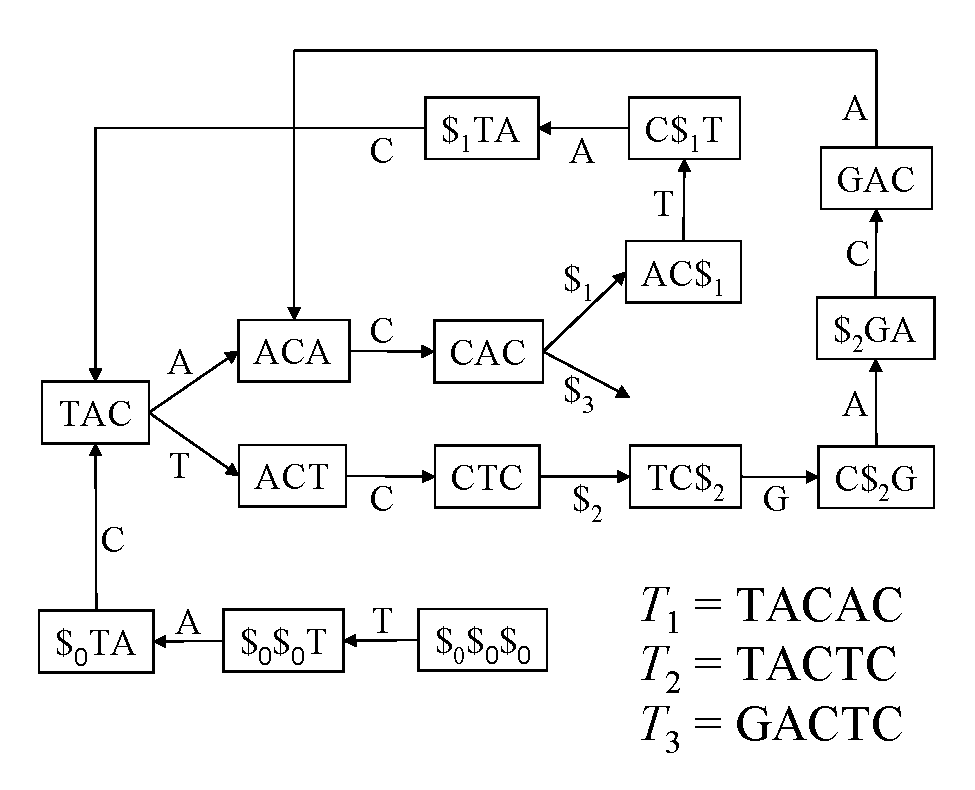
\includegraphics[scale=0.70]{fig3.eps} %PS
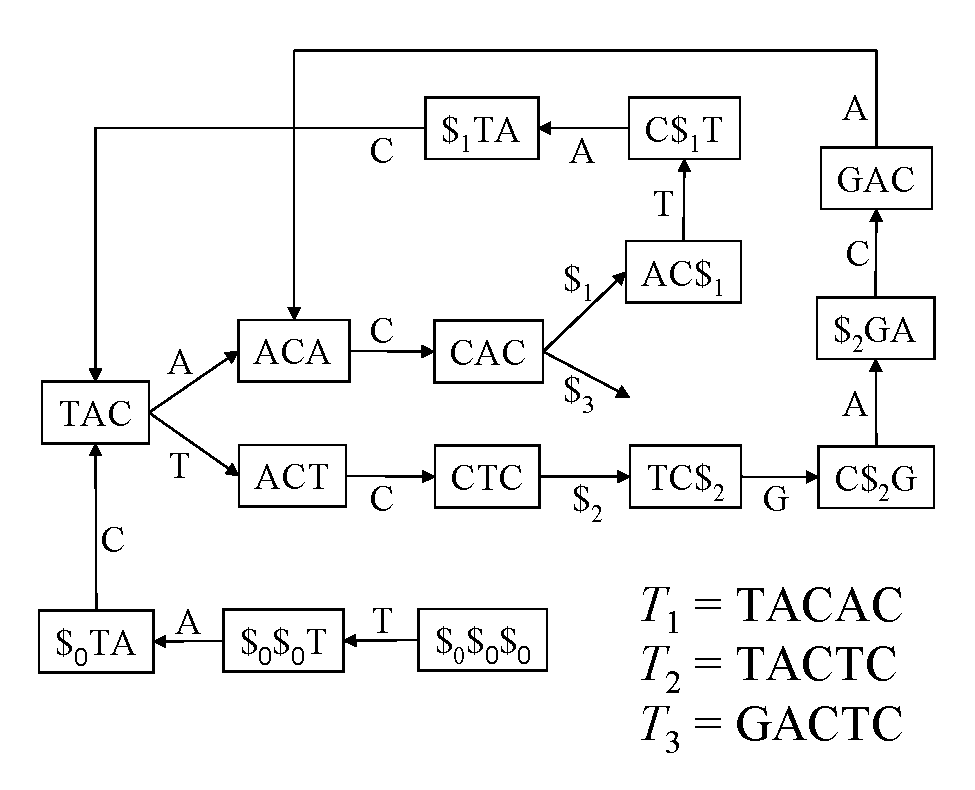
\includegraphics[scale=0.70]{fig3}
\caption{The $3$-dimensional de Bruijn graph of strings `TACAC', `TACTC', and
`GACTC'.}
\label{fig:debruijn}
\end{center}
\end{figure}

\cite{ICTFM12} introduced the {\em colored de Bruijn graph}, a variant of the classical structure, which is aimed at ``detecting and genotyping simple and complex genetic variants in an individual or population.'' The edge structure of the colored de Bruijn graph is the same as the classic structure, but now to each vertex ($(k - 1)$-mer) and edge ($k$-mer)
% FIXME: node coloring (CORTEX) looses information preserved in edge coloring(VARI), should we discuss this?  i.e. two nodes with the same color may or may not have a connecting edge with that color, but if you only color the nodes, you can't tell which is the case
is associated a list of colors corresponding to the samples in which the vertex or edge label exists. More specifically, given a set of $n$ samples, there exists a set $\mathcal{C}$ of $n$ colors $c_1, c_2, .., c_n$ where $c_i$ corresponds to sample $i$ and all $k$-mers and $(k-1)$-mers that are contained in sample $i$ are colored with $c_i$. A {\em bubble} in this graph corresponds to an undirected cycle, and is shown to be indicative of biological variation by \cite{ICTFM12}. 
{\sc Cortex}, the implementation of \cite{ICTFM12}, uses the colored de Bruijn graph to develop a method of assembling multiple genomes simultaneously, without losing track of the individuals from which $(k - 1)$-mers (and $k$-mers) originated. This graph is derived from either multiple reference genomes, multiple samples, or a combination of both.

Variant information of an individual or population can be deduced from structure present in the colored de Bruijn graph and the colors of each $k$-mer.
As implied by \cite{ICTFM12}, the ultimate intended use of colored de Bruijn graphs is to apply it to massive, population-level sequence data that is now abundant due to next generation sequencing technology (NGS) and multiplexing. These technologies have enabled production of sequence data for large populations, which has led to ambitious sequencing initiatives that aim to study genetic variation for agriculturally and bio-medically important species.  These initiatives include the {\em Genome 10K} project that aims to sequence the genomes of 10,000 vertebrate species~\citep{Haussler:2009}, the {\em iK5} project~\citep{Robinson:2011}, the 150 Tomato Genome ReSequencing project~\citep{tomato1,tomato2}, and the 1001 Arabidopsis project, a worldwide initiative to sequence cultivars of {\em Arabidopsis}~\citep{arabidopsis}.   Given the large number of individuals and sequence data involved in these projects, it is imperative that the colored de Bruijn graph can be stored and traversed in a space- and time-efficient manner.
 

\section{Rank and Select}
 \label{sec:rank} Two basic operations used in almost
every succinct and compressed data structure are {\em rank} and {\em select}.
Given a sequence (string) $S[1,n]$ over an alphabet $\Sigma =
\{1,\ldots,\sigma\}$, a character $c \in \Sigma $, and integers $i$,$j$,
$\rank_c(S,i)$ is the number of times that $c$ appears in $S[1,i]$, and
$\select_c(S,j)$ is the position of the $j$-th occurrence of $c$ in $S$.
%There is a great variety of techniques to answer these queries, with
%suitability depending on the nature of the sequence, for example, on whether or
%not it will be compressed and on the size of the alphabet.
For a binary string $B[1,n]$, the classic solution for rank and
select~\cite{Mun96} is built upon the input sequence, requiring $o(n)$
additional bits.  Generally, $\rank_1$ and $\select_1$ are considered the
default rank and select queries.  More advanced solutions
(e.g.~\cite{bitvector}) achieve zero-order compression of $B$,
%For example, the several structures (e.g.~\cite{bitvector}), (see
%also~\cite{kkp2014}), 
representing it in just $nH_0(B) + o(n)$ bits of space, and supporting $\rank$
and $\select$ operations in constant time. 
%Several practical implementations and improvements of RRR exists (see,
%e.g.,~\cite{kkp2014}).

\section{Wavelet Trees} \label{sec:WVT} To support rank and select on larger
alphabet strings, the wavelet tree~\cite{ggv2003,n2013} is a commonly used data
structure that occupies $n\log\sigma + o(n\log\sigma)$ bits of space and
supports $\rank$ and $\select$ queries in $\Oh{\log\sigma}$ time.  Wavelet trees
also support a variety of more complex queries on the underlying string (see,
e.g.~\cite{gnp2012}), in $\Oh{\log\sigma}$ time, and we will make use of some of
this functionality in Section~\ref{sec:implementing}.


%Our data structure for colored de Bruijn graphs is based on a succinct representation of individual de Bruijn graphs that was introduced by \cite{BOSS12} and which we refer to as the BOSS representation from the authors' initials.  The BOSS representation was in turn based on an adaptation of \cite{FM05} FM-indexes.  Before getting to our description of the succinct colored de Bruijn graph data structure, 
%In the rest of this section 
%we first describe FM-indexes and then explain the BOSS representation.
%Our explanation of BOSS is particularly simple and may be of independent interest to those wanting to better understand that data structure.
% This new take on BOSS was key to our development of our succinct colored de Bruijn graph. 
% Travis: No it wasn't, it came afterward. :o)

\section{FM-indexes}
\label{subsec:fm-indexes}

Consider a string $S$.  Let $F$ be the list of $S$'s characters sorted lexicographically by the suffixes starting at those characters, and let $L$ be the list of $S$'s characters sorted lexicographically by the suffixes starting immediately after those characters.  (The names $F$ and $L$ are standard for these lists.)  If \(S [i]\) is in position $p$ in $F$ then \(S [i - 1]\) is in position $p$ in $L$.  Moreover, if \(S [i] = S [j]\) then \(S [i]\) and \(S [j]\) have the same relative order in both lists; otherwise, their relative order in $F$ is the same as their lexicographic order.  This means that if \(S [i]\) is in position $p$ in $L$ then, assuming arrays are indexed from 0 and $\prec$ denotes lexicographic precedence, in $F$ it is in position
%\begin{multline*}
  \[|\{h\,:\,S [h] \prec S[i]\}| + |\{h\,:\,L [h] = S [i],\ h \leq p\}| - 1\,.\]
%  \end{multline*}
Finally, notice that the last character in $S$ always appears first in $L$.  It follows that we can recover $S$ from $L$, which is the famous Burrows-Wheeler Transform (BWT)~\citep{BW94} of $S$.

The BWT was introduced as an aid to data compression: it moves characters followed by similar contexts together and thus makes many strings encountered in practice locally homogeneous and easily compressible.  \cite{FM05} realized it could also be used for indexing because, if we know the range \(\BWT (S) [i..j]\) occupied by characters immediately preceding occurrences of a pattern $P$ in $S$, then we can compute the range \(\BWT (S) [i'..j']\) occupied by characters immediately preceding occurrences of \(c P\) in $S$, for any character $c$, since
\begin{eqnarray*}
i' & = & |\{h\,:\,S [h] \prec c\}| + |\{h\,:\,S [h] = c, h < i\}|\\
j' & = & |\{h\,:\,S [h] \prec c\}| + |\{h\,:\,S [h] = c, h \leq j\}| - 1\,.
\end{eqnarray*}
Notice \(j' - i' + 1\) is the number of occurrences of \(c P\) in $S$.  The essential components of an FM-index for $S$ are, first, an array storing \(|\{h\,:\,S [h] \prec c\}|\) for each character $c$ and, second, a rank data structure for \(\BWT (S)\) that quickly tells us how often any given character occurs up to any given position\footnote{Given a sequence (string) $S[1,n]$ over an alphabet $\Sigma = \{1,\ldots,\sigma\}$, a character $c \in \Sigma $, and an integer
$i$, $\rank_c(S,i)$ is the number of times that $c$ appears in $S[1,i]$.}.  
To be able to locate the occurrences of patterns in $S$ (in addition to just counting them), we can use a sampled suffix array of $S$ and a bitvector indicating the positions in \(\BWT (S)\) of the characters preceding the sampled suffixes.


\section{BOSS representation}
\label{sec:BOSS}

% TODO: take the concise description of BOSS from CDBG paper?

Conceptually, to build the BOSS representation~\cite{BOSS12} of a $K$th-order de Bruijn graph from a set of \((K + 1)\)-mers, we first add enough dummy \((K + 1)\)-mers starting with \$s so that if \(\alpha a\) is in the set, then some \((K + 1)\)-mer ends with $\alpha$ ($\alpha$ a $K$-mer, $a$ a symbol).  We also add enough dummy \((K + 1)\)-mers ending with \$ that if \(b \alpha\) is in the set, with $\alpha$ containing no \$ symbols, then some \((K + 1)\)-mer starts with $\alpha$.  We then sort the set of \((K + 1)\)-mers into the right-to-left lexicographic order of their first $K$ symbols (with ties broken by the last symbol) to obtain a matrix.  If the $i$th through $j$th \((K + 1)\)-mers start with $\alpha$, then we say node \([i, j]\) in the graph has label $\alpha$, with \(j - i + 1\) outgoing edges labelled with the last symbols of the $i$th through $j$th \((K + 1)\)-mers.  If there are $n$ nodes in the graph, then there are at most \(\sigma n\) rows in the matrix, i.e., \((K + 1)\)-mers.

For example, if \(K = 3\) and the matrix is the one from Bowe et al.'s paper,
shown in the left of Fig.~\ref{fig:matrix}, then the \(n = 11\) nodes are
\begin{gather*}
 [1, 1], [2, 2], [3, 3], [4, 5], [6, 6], [7, 7], [8, 9], [10,
 10], [11, 11], \\ [12, 12], [13, 13]
\end{gather*}
with labels

\begin{gather*}
 \mathrm{\$\$\$}, \mathrm{CGA}, \mathrm{\$TA}, \mathrm{GAC}, \mathrm{TAC},
\mathrm{GTC}, \mathrm{ACG}, \mathrm{TCG}, \mathrm{\$\$T}, \\
\mathrm{ACT}, \mathrm{CGT},
\end{gather*}%
respectively. The 3rd-order de Bruijn graph itself is shown in the right of the figure.

\begin{figure*}[!t]
\centering
\begin{tabular}{c@{\hspace{10ex}}c}
\begin{tabular}{r@{\hspace{1ex}}@{\hspace{1ex}}@{\hspace{1ex}}l@{\hspace{1ex}}c}
1) & \,\$\,\$\,\$\, & T\\
2) & CGA & C\\
3) & \,\$\,TA & C\\
4) & GAC & G\\
5) & GAC & T\\
6) & TAC & G\\
7) & GTC & G\\
8) & ACG & A\\
9) & ACG & T\\
10) & TCG & A\\
11) & \,\$\,\$\,T & A\\
12) & ACT & \$\\
13) & CGT & C
\end{tabular} &
\raisebox{-10ex}
{\includegraphics*[trim = 0cm 0cm 9cm 24cm, width=50ex]{images/dbg-with-dummies.pdf}}
\end{tabular}
\caption{The BOSS matrix (left) and de Bruijn graph (right) for the quadruples CGAC, GACG, GACT, TACG, GTCG, ACGA, ACGT, TCGA, CGTC.}
\label{fig:matrix}
\hrulefill
\end{figure*}

Bowe et al.\ described a number of queries on the graph, all of which can be implemented in terms of the following three with at most an $\Oh{\sigma}$-factor slowdown:
\begin{itemize}
\item $\forward(v, a)$ returns the node $w$ reached from $v$ by an edge labelled $a$, or NULL if there is no such node;
\item $\backward(v)$ lists the nodes $u$ with an edge from $u$ to $v$;
\item $\lastchar(v)$ returns the last character of $v$'s label.
\end{itemize}
In our example, \(\forward \allowbreak ([8, 9], \mathrm{A}) \allowbreak =
\allowbreak [2, 2]\),
\(\backward \allowbreak ([2, 2]) \allowbreak = \allowbreak [8, 9], [10, 10]\) and
\(\lastchar \allowbreak ([8, 9]) \allowbreak = \allowbreak \mathrm{G}\).
Since $\backward$ always returns at least one node, we can recover any non-dummy node's entire label by $K$ calls to $\lastchar$ interleaved with \(K - 1\) calls to $\backward$.




\section{Varying order}
\label{sec:changing}

If we delete the first column of the matrix in Figure~\ref{fig:matrix}, the result is {\em almost} the BOSS matrix for a 2nd-order de Bruijn graph whose nodes
\[[1, 1], [2, 2], [3, 3], [4, 6], [7, 7], [8, 10], [11, 11], [12, 12], [13, 13]\]
have labels
\[\mathrm{\$\$, GA, TA, AC, TC, CG, \$T, CT, GT}\,,\]
respectively.  Similarly, if we delete the first two columns of the original matrix, the result is almost the BOSS matrix for a 1st-order graph whose nodes
\[[1, 1], [2, 3], [4, 7], [8, 10], [11, 13]\]
have labels
\[\mathrm{\$, A, C, G, T}\,,\]
respectively.  If we delete the first three columns, the result is almost the BOSS graph for the 0th-order graph whose single node \([1, 13]\) has an empty label.  Notice we allow the same node to appear in different graphs, with labels of different lengths.  If readers find this confusing, they can imagine that nodes are triples instead of pairs, with the additional component storing the label's length.

The truncated form of a higher order BOSS differs from the BOSS of a lower order in that
%The problem is that 
some rows are repeated, which could prevent the BOSS representation from working properly.  Suppose that, instead of trying to apply $\forward$, $\backward$ and $\lastchar$ directly to nodes in the new graphs, we augment the BOSS representation of the original graph to support the following three queries:
\begin{itemize}
\item $\shorter(v, k)$ returns the node whose label is the last $k$ characters of $v$'s label;
\item $\longer(v, k)$ lists nodes whose labels have length \(k \leq K\) and end with $v$'s label;
\item $\maxlen(v, a)$ returns some node in the original graph whose label ends with $v$'s label, and that has an outgoing edge labelled $a$, or NULL otherwise. %if there is no such node.
\end{itemize}
If we want a node in the original graph whose label ends with $v$'s label but we do not care about its outgoing edges, then we write \(\maxlen(v, *)\).  Notice $\shorter$ and $\longer$ are symmetric, in the sense that if $v$'s label has length $k_v$ and \(x \in \longer(v, k_v)\), then \(\shorter(x, k_v) = v\).  In our example, \(\shorter([4, 5], 2) = [4, 6]\) while \(\longer([4, 6], 3) = [4, 5], [6, 6]\) and \(\maxlen ([4, 6], \mathrm{G})\) could return either \([4, 5]\) or \([6, 6]\), while \(\maxlen([4, 6], \mathrm{T}) = [4, 5]\) and \(\maxlen([4, 6], \mathrm{A}) = \mathrm{NULL}\).

If $v$ is a node in the original graph --- e.g., $v$ is returned by $\maxlen$ --- then we can use the BOSS implementations of $\forward$, $\backward$ and $\lastchar$.  Otherwise, if $v$'s label has length $k_v$ then
\begin{eqnarray*}
\forward(v, a) & = & \shorter(\forward(\maxlen(v, a), a), k_v)\\
\lastchar(v) & = & \lastchar(\maxlen(v, *))\,.
\end{eqnarray*}
Assuming queries can be applied to lists of nodes, we can compute \(\backward(v)\) as %by computing
\[\shorter(\backward(\maxlen(\longer(v, k_v + 1), *)), k_v),\]
removing any duplicates.

To see why we can compute $\backward$ like this, suppose $v$'s label is \(\alpha a\), so \(\longer(v, \allowbreak k_v + 1)\) returns a list of all \(d \leq \sigma\) nodes whose labels have the form \(b \alpha a\).  Applying $\maxlen$ to this list returns a second list of $d$ nodes, with labels \(\beta_1 b_1 \alpha a, \ldots, \beta_d b_d \alpha a\) of length $K$.  Applying $\backward$ to this second list returns yet a third list, of all the at most \(\sigma d\) nodes whose labels have the form \(c \beta_i b_i \alpha\).  We need only one node returned calling $\backward$ on each node in the second list, so we can discard all but at most $d$ nodes in the third list.  Finally, applying $\shorter$ to the third list returns a fourth list, of all $d$ nodes whose labels have the form \(b_i \alpha\), each of which may be repeated at most $\sigma$ times in the list.



\section{Implementing $\shorter$, $\longer$ and $\maxlen$}
\label{sec:implementing}

The BOSS representation includes a wavelet tree over the last column $W$ of the BOSS matrix, and a bitvector $L$ of the same length with 1s marking where nodes' intervals end.  In our example, \(W = \mathrm{TCCGTGGATAA\$C}\) and \(L = 1110111011111\).

%With these data structures, 
Now we can implement \(\maxlen([i, j], a)\) in $\Oh{\log \sigma}$ time: we use $\rank$ and $\select$ on $W$ to find an occurrence \(W [r]\) of $a$ in \(W [i..j]\), if there is one; we then use $\rank$ and $\select$ on $L$ to find the last bit \(L [i' - 1] = 1\) with \(i' \leq r\) and the first bit \(L [j'] = 1\) with \(j' \geq r\), and return \([i', j']\).  (If there is no occurrence of 1 strictly before \(L [r]\), then we set \(i' = 1\).)  We can implement \(\maxlen([i, j], *)\) in $\Oh{1}$ time: instead of using $\rank$ and $\select$ on $W$ to find $r$, we simply choose any $r$ between $i$ and $j$.

In our example, for \(\maxlen([4, 6], \mathrm{G})\) we first find an occurence \(W [r]\) of G in \(W [4..6]\), which could be either \(W [4]\) or \(W [6]\); if we choose \(r = 4\) then the last bit \(L [i' - 1] = 1\) with \(i' \leq r\) is \(L [3]\) and the first bit \(L [j'] = 1\) with \(j' \geq r\) is \(L [5]\), so we return \([i', j'] = [4, 5]\); if we choose \(r = 6\) then the last bit \(L [i' - 1] = 1\) with \(i' \leq r\) is \(L [5]\) and the first bit \(L [j'] = 1\) with \(j' \geq r\) is \(L [6]\), so we return \([i', j'] = [6, 6]\).

To implement $\shorter$ and $\longer$, we store a wavelet tree over the sequence $L^*$ in which \(L^* [i]\) is the length of the longest common suffix of the label of the node in the original graph whose interval includes $i$, and the label of the node whose interval includes \(i + 1\); this takes $\Oh{\log K}$ bits per \((K + 1)\)-mer in the matrix.  To save space, we can omit $K$s in $L^*$, since they correspond to 0s in $L$ and indicate that $i$ and \(i + 1\) are in the interval of the same node in the original graph; the wavelet tree then takes $\Oh{\log K}$ bits per node in the original graph and $\Oh{n \log K}$ bits in total.  In our example, \(L^* = 0, 1, 0, 3, 2, 1, 0, 3, 2, 0, 1, 1\) (and we can omit the 3s to save space).

For \(\shorter([i, j], k)\), we use the wavelet tree over $L^*$ to find the largest \(i' \leq i\) and the smallest \(j' \geq j\) with \(L^* [i' - 1], L^* [j'] < k\) and return \([i', j']\), which takes $\Oh{\log K}$ time.  For \(\longer([i, j], k)\), we use the wavelet tree to find the set \(B = \{b\,:\,L^* [b] < k\,;\,i - 1 \leq b \leq j\}\) --- which includes \(i - 1\) and $j$ --- and then, for each consecutive pair \((b, b')\) in $B$, we report \([b + 1, b']\); this takes a total of $\Oh{|B| \log K}$ time.  With these implementations, if the time bounds for \(\forward(v, a)\), \(\backward(v)\) and \(\lastchar(v)\) are $\Oh{t_\forward}$, $\Oh{t_\backward}$ and $\Oh{t_\lastchar}$ when $v$ is a node in the original graph, respectively, then they are $\Oh{t_\forward + \log \sigma + \log K}$, $\Oh{\sigma (t_\backward + \log K)}$ and $\Oh{t_\lastchar + 1}$ when $v$ is not a node in the original graph.

In our example, for \(\shorter([4, 5], 2)\) we find the largest \(i' \leq 4\) and the smallest \(j' \geq 5\) with \(L^* [i' - 1], L^* [j'] < 2\) --- which are 4 and 6, respectively --- and return \([4, 6]\).  For \(\longer([4, 6], 3)\) we find the set \(B = \{b\,:\,L^* [b] < 3\,;\,3 \leq b \leq 6\} = \{3, 5, 6\}\) and report \([4, 5]\) and \([6, 6]\).

A smaller but slower approach is not to store $L^*$ explicitly but to support access to any cell \(L^* [i]\) by finding the nodes in the original graph whose intervals include $i$ and \(i + 1\), then using $\backward$ and $\lastchar$ to compute their labels and find the length of their longest common suffix; this takes a total of $\Oh{K (t_\backward + t_\lastchar)}$ time.  To implement $\shorter$ and $\longer$, we store a range-minimum data structure~\cite{fh2011} over $L^*$, which takes \(2 n + o (n)\) bits and returns the position of the minimum value in a specified substring of $L^*$ in $\Oh{1}$ time.

For \(\shorter([i, j], k)\), we use binary search and range-minimum queries to find the largest \(i' \leq i\) and the smallest
\(j' \geq j\) with \(L^* [i' - 1], L^* [j'] < k\) and return \([i', j']\), which takes $\Oh{K (t_\backward + t_\lastchar) \log (n \sigma)}$ time. 
%(With a more complicated use of the range-minimum data structure, which we will describe in the full version of this paper, we use $\Oh{K^2 (t_\backward + t_\lastchar)}$ time.)
For \(\longer([i, j], k)\), we recursively split \([i, j]\) into subintervals with range-minimum queries, at each step using $\backward$ and $\lastchar$ to check that the minimum value found is less than $k$; this takes $\Oh{K (t_\backward + t_\lastchar)}$ time per node returned.  With these implementations, \(\forward(v, a)\), \(\backward(v)\) and \(\lastchar(v)\) take $\Oh{t_\forward + K (t_\backward + t_\lastchar) \log (n \sigma)}$, $\Oh{\sigma K (t_\backward + t_\lastchar) \log (n \sigma) + \sigma^2 t_\backward}$ and $\Oh{t_\lastchar + 1}$ time, respectively, when $v$ is not a node in the original graph.

For \(\sigma = \Oh{1}\), our bounds are summarized in the following theorem. % We will provide more details in the full version of this paper.

\begin{theorem}
\label{thm:bounds}
When \(\sigma = \Oh{1}\), we can store a variable-order de Bruijn graph in $\Oh{n \log K}$ bits on top of the BOSS representation, where $n$
is the number of nodes in the $K$th-order de Bruijn graph, and support \forward\ and \backward\ in $\Oh{\log K}$ time and \lastchar\ in
$\Oh{1}$ time.  We can also use $\Oh{n}$ bits on top of the BOSS representation, at the cost of using $\Oh{K \log n / \log \log n}$ time
for \forward\ and \backward.
\end{theorem}

%shorter - logK
%longer - |B| log K time (for a set of B resulting nodes)

%K^2 log^2 n / log log n

%O(B K^2 log^2 n / log log n)

\chapter{Experimental Analysis}
\label{sec:experiments}

\section{Implementation}
SDSL-lite, STXXL for the implementation of on disk sorting, which also lets the user specify the work to be done in memory.

%\section{Primary vs Secondary memory construction}
%In memory, single IDE disk, single SSD, 2 SSDs, 4 SSDs.
%Cost effective? SSD vs memory cost.

\section{BOSS vs Competing methods}
Construction time, bits per edge, and traversal time for 2 small genomes.
(would have to implement simple traversal for this)

\section{Variable-order vs fixed-order}
\input{chapters/experiments-varord.tex}


%%%%%%%%%%%%%%  PS
\section{Cortex vs Vari}
%Measure full runtime of both.
%Test w/ on disk colour matrix? (sort indices after traversal)
\pyt{Remove the initial 2 sentences? I.e. Measure full runtime of both...}


We evaluated $\ours$ on five different datasets, described below.  For performance evaluation, we compare peak memory, which was measured as the maximum resident set size, and runtime, measured as the user process time as our metrics.  In addition to evaluating performance, we also validated $\ours$ by the ability to correctly call bubbles and to accurately identify the origin of $k$-mers in a simulated metagenomics sample.  Finally, we present observations computed by $\ours$ on a collection of metagenomic samples taken from commercial beef production facilities.



\subsection{Datasets} \label{data}

Five different datasets were chosen in order to test and evaluate $\ours$ on a variety of diverse yet realistic data types that are likely to be used as input into $\ours$.  The first dataset contained six sub-strains of the {\em E. coli} K-12 strain reference genomes from NCBI.  The accession and substrains are 	AP009048 -- W3110,  
	CP009789 -- ER3413, 
	CP010441 -- ER3445, 
	CP010442 -- ER3466, 
	CP010445 -- ER3435, and 
	U00096   -- MG1655. 
    Each of the genomes contained approximately 4.6 million base pairs and had a median GC content of 49.9\%.

% (\ref{tbl-ecoli}).


    
%% \begin{table}[h!]
%%   \small
%%   \centering
%%   \begin{tabular}{c|c|c}
%% 		{\bf Accession Number}		& {\bf Sub-strain}	& {\bf Genome Size} 	 \\
%% 	\hline
%% 	\hline
%% 	AP009048 & W3110  & 4,646,332 bp \\
%% 	CP009789 & ER3413 & 4,558,660 bp \\
%% 	CP010441 & ER3445 & 4,607,634 bp \\
%% 	CP010442 & ER3466 & 4,660,432 bp \\
%% 	CP010445 & ER3435 & 4,682,086 bp \\ 
%% 	U00096   & MG1655 & 4,641,652 bp\\
%%  	\end{tabular}
%%       \caption{Characteristics of the substrains of \emph{E. coli} K-12 used to test the performance and accuracy of $\ours$}.
%%  \label{tbl-ecoli}
%% \end{table}

Our second dataset was composed of reference genomes for four different plant species: \emph{Oryza sativa Japonica} (rice, NCBI Accession numbers: NC\_008394 to NC\_008405), \emph{Solanum lycopersicum} (tomato, NCBI Accession numbers: NC\_015438 to NC\_015449),  \emph{Zea mays} (corn, NCBI Accession numbers: NC\_024459 to NC\_024468), and  \emph{Arabidopsis thaliana} (Arabidopsis, [NCBI Accession numbers: NC\_003070 to NC\_003076).  The genome sizes and GC content were 430 Mbp and 43.42\% \citep{rice}, 950 Mbp and 43.42\% \citep{tomato1,tomato2}, 2.07 Gbp and 35.70\% \citep{corn}, and 135 Mbp and 47.4\% \citep{swarbreck}, respectively.  Hence, this represents a significantly larger dataset with more varied GC content than the {\em E. coli} dataset, and therefore placed more demands on both the performance and accuracy of $\ours$.  


%% \begin{table}[h!]
%%   \small
%%   \centering
%%   \begin{tabular}{c|c|c}
%% 		{\bf AMR Gene}&{\bf Resistance Type}&{\bf Accession Number} 	 \\
%% 	\hline
%% 	\hline
%% 	AmpH & beta-lactamase & AFQ67211 \\
%% 	OKP-B-4 & beta-lactamase & CAJ19612 \\
%% 	NDM-6 & beta-lactamase  & AEX08599 \\
%% 	MAL-1 & beta-lactamase & CAC33434  \\
%% 	MOX-2 & beta-lactamase  & CAB82578  \\
%% 	TLA-1 & beta-lactamase & ADM26831   \\
%% 	SED-1 & beta-lactamase  & AAK63223   \\
%% 	TEM-1& beta-lactamase  & AFI61435   \\
%% 	TET-X & Tetracycline & AAA27471   \\
%% 	TET-X(1) & Tetracycline  & ADD83116 \\
%% 	TET-C & Tetracycline  & NP\_387454  \\
%% 	TETR-G & Tetracycline & AAB24797 \\
%%  	\end{tabular}
%%       \caption{List of AMR genes used to generate the simulated sample. The first seven genes were included in the the 54 beta-lactamase genes we considered for this experiment, and the remaining four were tetracycline genes. Each of the genes were approximately 1,000 bp in length and had varied GC content.}
%%  \label{tbl-amr}
%% \end{table}








Our third dataset consists of the set of all 3,765  NCBI GenBank assemblies having the organism\_name field equal to ``Escherichia coli'' as of March 22, 2016.  The union of all assemblies contains 155,449,228 31-mers.  The minimum, maximum, and average assembly lengths are 2,911,360 bp, 7,687,202 bp, and 5,156,744 bp, respectively.  The average GC content is 50.5\%. 

As previously described, our fourth dataset contains 54 beta-lactamase genes from a custom database and a simulated metagenomics sample.  We first compiled a database of known AMR genes based on sequences in the databases CARD \citep{mcarthur}, Resfinder \citep{zankari} and ARG-ANNOT \citep{gupta}---each of these AMR-specific databases are actively curated and contain the genetic sequences for a large variety of AMR genes.  This database contains all known AMR genes, their drug resistance, and mechanism conferring resistance.  We selected 54 beta-lactamase genes from this database that are known to have very high clinical and public health importance, and simulated 26,516,559 paired-end 120 bp reads from seven of the 54 beta-lactamase genes (Accession numbers AFQ67211, CAJ19612, AEX08599, CAC33434, CAB82578, ADM26831, AAK63223, and AFI61435), as well as four additional AMR genes that were not included in this set of 54 genes (Accession numbers AAA27471, ADD83116, NP\_387454, and AAB24797).  These latter four genes were tetracycline-resistant genes.  Tetracyclines are a group of broad-spectrum antibiotics and hence, their resistance is also clinically important.   This AMR dataset was used not only in the memory and time performance but also used to test the ability of $\ours$ in identifying beta-lactamase genes from a typical metagenomic sample containing a variety of AMR genes.  %Table \ref{tbl-amr} contains the gene name, resistance type (beta-lactamase or  tetracycline), and accession number of 11 genes that were used in simulation of the sample. 


Our fifth dataset consists of 87 metagenomic samples taken from various locations along the production process for eight pens of cattle in two beef production facilities by \cite{noyes2016resistome}.  These locations were feedlot arrival, feedlot exit, transport truck, slaughter holding (arrival), and slaughter trimmings and sponges (exit).  Samples were arranged into groups based on these locations. These samples were collected to explore the hypothesis that widespread use of antimicrobial drugs (administered with livestock feed for these samples) introduce selective pressure on microbial communities and thus foster the evolution of antimicrobial resistant bacteria.  These antimicrobial resistant bacterial are important because they present a public health risk.  In addition to the metagenomic samples, we included 4,062 AMR genes from the previously mentioned gene databases.  23 genes in the databases containing IUPAC codes other than the four bases were filtered out as KMC2 and the succinct de Bruijn graph were configured with a four symbol alphabet.  The union of all samples and genes contains 40,995,794,366 32-mers and the GC content is 44.3\%.





% software configuration
We ran our experiments with the following configuration and environment.  On the {\it E. coli} reference, plant, and simulated metagenomic datasets we ran $\ours$ with RRR encoding, without external construction, and used {\sc Cortex} as the front end to generate the uncompressed $k$-mer union and colors.  On the {\it E. coli} assembly dataset, we ran $\ours$ similarly but used the KMC2 front end and our streaming based set-union construction.  On the metagenomic sample, we ran $\ours$ with the KMC2 front end, online Elias-Fano encoding for $C$, and external BOSS construction.
% hardware configuration
The first, second, and fourth experiments were performed on a 2 Intel Xeon  E5-2650 v2 server with 386 GB of RAM, and both resident set size and user process time were reported by the operating system.  The third experiment was performed on an AMD Opteron  6220  with 512 GB of RAM and 32 cores.  The fifth experiment was performed on an AMD Opteron 6378  with 512 GB of RAM and 64 cores. 

\subsection{Time and Memory Usage}

% what is bubble calling
To compare $\ours$ resource use with {\sc Cortex} by \cite{ICTFM12}, we constructed the colored de Bruijn graph for the {\it E. coli} reference dataset, the four plant assembly dataset, and the simulated AMR dataset, then performed {\em bubble calling} on all three data structures,  and recorded the peak memory usage and runtime.    Resource comparison with {\sc Cortex} was only possible on the smaller three datasets, as the largest two have too many $k$-mers and colors to fit in memory on our machines with {\sc Cortex}.  Based on the data structure defined in {\sc Cortex}'s source as well as the supplementry information provided by Iqbal {\it et al.}, it would have required $>$ 3 TB of RAM and $>$ 18 TB of RAM for its hash table entries alone, respectively.




% construction statistics
%For the {\it E. coli} assembly dataset, after $k$-mer counting with KMC2, construction took 16 hours and 387 GB of RAM for this dataset. For the beef safety samples, it took KMC2 34 hours and 12 GB of RAM to $k$-mer count the 887 GB of trimmed reads. $\ours$ required 87 hours, 218 GB of RAM, and 4.4 TB of external memory to build the succinct colored de Bruijn graph.  The uncompressed $C$ temporary file was 1.4 TB in size, which compressed to 196 GB with Elias-Fano encoding.



%For the simulated metagenomic dataset, each AMR gene was assigned a separate color allowing the match-color algorithm to be applied.  Thus no graph traversal times are reported although the size of the structures are reported.  
%We ran the bubble calling algorithm between the colors for the assemblies ``GCF\_000005845.2\_ASM584v2\_genomic'' and ``GCF\_000006665.1\_ASM666v1\_genomic''.

%% On the final two datasets, the simulated metagenomic sample and beef safety samples, we are interested in detecting the presence of known AMR genes among the reads.  
%% we explore the feasibility of using a colored de Bruijn graph for AMR gene detection among metagenomic samples.
%% We do so by visiting $k$-mers found in AMR genes and look for those that co-occur in the metagenomic samples.

%% % discussion of k-mer intersection
%% On the final two datasets, instead of using either of {\sc Cortex}'s bubble calling algorithms, which are designed for variant detection we are interested in presence of the AMR genes in the sample.  Variants may represent read errors or largely homologous genes missing the antibiotic resistant determinant. in samples taken from a pair of individuals or individual and reference,   In this applications, instead of looking for variants, we are looking for similarity
%% % varants -- regions that differ flanked by homologous regions, we are looking strictly for homologous regions -- as the metagenomic sample may be plagued with incomplete coverage
%% in the presence of incomplete coverage, a mix of many individuals, thus weakening common read error correction assumptions, and significant homology among AMR genes and their possibly co-occuring ancestral variants leading to more tangled graphs which impair {\sc Cortex}'s cleaned individual oriented algorithm.  In the absence of a colored, metagenomic-aware traversal algorithm, we focus only on regions of similarity and allow unlimited sized gaps between them, where the metagenomic sample color may be highly tangled or unconnected.  

%% One thing that distinguishes such datasets from pangenomic datasets, such as those targeted by the bloom filter trie, is that these datasets may have significantly smaller amounts of redundancy.  On the beef safety dataset, for example, two thirds of $k$-mers occur with multiplicity of one across the whole collection.  

%% On the simulated metagenomic dataset, 

%% For the $k$-mer set operation was not necessary and no time comparison is reported.

%% Hence this experiment demonstrates the viability of AMR gene detection via $k$-mer set operations.

%% For the 87 metagenomic sample dataset, the full data structures were loaded in memory, however only the length of each gene sequence need be traversed, resulting in the relatively fast 21 minute load and traverse time compared with bubble calling across a genome.


%% On the 87 beef safety sample, we implemented a variant of {\sc Cortex}'s path divergence algorithm, which locates bubbles where one arm of the bubble is allowed to have branches because its path is guided by a reference sequence.  In our version, we traverese the walk specified by each AMR gene sequence and count the number of edges shared with all samples from each sample location in the beef production pipeline.  


%% We note the benefit  of using a rank-select capable dictionary datastructure such as RRR or Elias-Fano encoded bit vector and storing the color matrix in linearized row major order.  Samples were arranged such that all samples taken from the same location within the production process were placed in consecutive columns in $C$.
%% %To analyze colored de Bruijn graphs with {\sc Cortex}'s algorithms, we must do all pairs comparisons or at least compare every sample of interest against some reference color; both of which become a growing runtime burden as the number of colors increases.
%% In this configuration, our data structure allows us to work on groups of samples at a time while still maintaining each sample individuality for analyses when that is of interest.  Specifically, if colors are ordered by relevant groups, such as by  the location samples were taken in the beef production pipeline.  With such grouping, we can count the number of sample colors from a group that are present in a given edge quickly.  This is computed in constant time as the difference between rank queries on the group's column interval bounds.

In order to test performance characteristics, various experiments were performed on all five datasets described in the previous subsection.  Datasets varied in the number of $k$-mers in the graph from four million to over 40 billion.  As can be seen in Table \ref{tbl-cosmo}, where directly comparable, $\ours$ used less than one-fifth of the peak memory that {\sc Cortex}  required but required greater running time.  This memory and time trade-off is important in larger population level data.  %Given that {\sc Cortex} requires 100.93 GB of space for four plant species, it would be perceptibly infeasible to run it on the i5K initiative dataset that contains the genetic sequence data for 5,000 insect species.
This is highlighted by our largest two datasets which could not be run with {\sc Cortex}.
Hence, lowering the memory usage in exchange for higher running time deserves merit in contexts where there is data from large populations. 
 
%We note that the ratios were greater for the AMR dataset, which was likely due to the greater number of colors in the AMR versus the \emph{E. coli} and plant datasets (55 versus 6 and 4, respectively).


\begin{table*}%[h!]
  \small
  \centering
  \begin{tabular}{| l | r | r | c | c | c |c |}
   	\hline
	\multicolumn{1}{|l}{}
   	& \multicolumn{1}{r}{}	
	& \multicolumn{1}{r}{} 
	& \multicolumn{2}{c|}{{\sc Cortex}} 
	& \multicolumn{2}{|c|}{$\ours$}  \\
	\hline
	 Dataset & No. of $k$-mers & Colors & Memory & Time & Memory & Time \\
	\hline
	\emph{E. coli} reference genomes			& 4,627,104 		& 6 	& 363.64 MB 	& 9 s 	& 72.38 MB  	& 1m 19s\\
	Plant reference genomes					& 1,621,663,030 	& 4 	& 100.93 GB 	& 2h 18m	& 19.46 GB 	& 17h 28m\\
    NCBI \emph{E. coli} assemblies          & 155,449,228       & 3,765 & N/A        & N/A      &  26.50 GB      & 11h \\
	AMR genes and sample 					& 9,348,365 		& 55 	& 7.08 GB 	& 2m 55s	& 0.718 GB 	& 29m 21s \\ 
    Beef safety                             & 40,995,794,366    & 88    & N/A        & N/A   & 245 GB     & N/A \\
 	\hline
	\end{tabular}
  \caption{Comparison between the peak memory and time usage required to store all the $k$-mers and run bubble calling on the data in {\sc Cortex} and $\ours$.
    %$k= 31$ was used for all datasets.
    The peak memory is given in megabytes (MB) or gigabytes (GB). The running time is reported in seconds (s), minutes (m), and hours (h).}
 \label{tbl-cosmo}
\end{table*}

\subsection{Validation on E. coli Genomes}

In order to validate our data structure and test the accuracy of the bubble calling method of $\ours$, we compared the bubbles found by running the bubble calling algorithm on the \emph{E. coli} reference dataset using {\sc Cortex} and $\ours$.  The bubbles outputted by each method were compared by identifying the flank preceding each bubble.  Both $\ours$ and {\sc Cortex} identified 465 bubbles across all six \emph{E. coli} K-12 substrains.  This number accounts for the reverse complement bubbles found by $\ours$. The methods agree on 98.5\% (458 / 465) of the bubbles. Thus, $\ours$ found seven bubbles that were not identified by {\sc Cortex}, which were shown to be valid, and {\sc Cortex} found seven bubbles not identified by $\ours$.
% I'm commenting this next line out because it doesn't make sense; cortex stores connonical k-mers, so implicitly has revcomps too.
% These latter bubbles were missed by $\ours$ because the addition of the reverse complement adds complexity to the graph, which changes these regions from containing a single bubble to a more complex structure.
Nonetheless, our validation shows that 98.5\% of the variation determined by {\sc Cortex} and $\ours$ is identical.

\subsection{Validation on AMR Dataset}

Next, we validated the ability of $\ours$ to correctly identify the AMR genes contained in a metagenomics sample using a set of reference genes. $\ours$ constructed the colored de Bruijn graph from the set of 54 beta lactamases and the simulated metagenomics sample. Hence, there were 55 unique colors in the graph because there exists one color for the metagenomic sample and one unique color for each of the 54 beta-lactamase genes.  Next, for each of the 54 genes, the unique $k$-mers were identified and the total number of these $k$-mers that were contained in the simulated sample was determined.  

%Table \ref{amr2} in the Supplement gives the total number of each unique $k$-mers for each gene, the number of these $k$-mers that were found in the simulated reads, and the {\em shared k-mer fraction} that is defined by the division of the two numbers.
The shared $k$-mer fraction for each of the 54 genes ranged from 0.41 to 1 with a mean of 0.62.  All of the seven beta-lactamase genes that were contained in the simulated sample had a shared $k$-mer fraction of 1, whereas none of the remaining 47 genes did.  Of the 47 beta-lactamase genes that were not contained in the simulated sample, two had a shared $k$-mer fraction 0.98 and 0.95, however, these genes had 97\% and 95\% sequence similarity to one of the seven genes contained in the sample.  All the remaining 45 genes had a shared $k$-mer fraction between 0.79 and 0.41.  Hence, this demonstrates (on a small scale) that this use of the colored de Bruijn graph and our match color algorithm is a viable method to identify AMR genes in a metagenomics sample. 

\subsection{Observations on Beef Safety Dataset}

%While the primary purpose of this experiment is to measure the performance in terms of memory footprint, we can examine the data we collected during traversal which may be useful to biologists and spawn hypotheses for further investigation.
Finally, we used $\ours$ to make observations about the presence of AMR genes in the beef safety dataset.  As previously described, during out path divergence derived algorithm, we compute a count of how many $k$-mers in each AMR gene are found across all samples within a sample group.  This algorithm need only traverse the AMR genes, so despite the size of the overall dataset, it only took 21 minutes to load and access the necessary parts of the data structure.  In contrast, if bubble calling were to run at the same rate for this dataset as for the {\it E. coli} assembly dataset, it would take 3,001 hours to complete, thus suggesting a need for a targeted inquiry approach on datasets of this size.  

Since longer genes have more $k$-mers, the counts are likely to be larger, as are those from larger sample groups.  To make these counts comparable, we normalize by both gene length and sample group size.  We can then examine the number of genes having a disproporitionately large ($>$ 3 std. dev. above mean) shared $k$-mer count for each gene and sample group combination.  The number of such genes with disproporitionately large normalized counts in each sample group were:  feedlot arrival --- 304, feedlot exit --- 93, transport truck --- 230, slaughter holding (arrival) --- 16, and slaughter trimmings and sponges (exit) --- 0.
%Despite biases in the sampling process that need to be taken into account for substantial biological implications, one validating property of these observations is that there were no AMR genes with disproporitionately large representation in the samples taken on exit from the slaughter location.
This observation supports the conclusion of \cite{noyes2016resistome}, namely, that antimicrobial interventions during slaughter were effective in reducing AMR gene presence in the finished product. 

%\subsection{Hypotheses}
%\subsection{Method}
%\subsection{Test Data}
%\label{sec:data}

\section{Discussion and Conclusions} \label{sec:discussion} 

%To the best of our knowledge, t
This paper describes the first non-proprietary computational method for identifying misassembly errors using short read sequence data and optical mapping data.
% has not been previously considered using non-proprietary software.  
 Our results demonstrate: (1) a substantial number of misassembly errors can be identified in draft genomes of prokaryote and eukaryote speices; (2) our method scales to large genomes; and (3) it can be used in combination with any
 assembler and thus, making it a viable post-processing step for any assembly. 

While $\sequel$ is capable of identifying a significant percentage of misassembly errors, it does not address 
%the additional problem of re-assembling 
the reassembly of those the misassembled contigs. 
Correcting misassembly errors by segmenting the contigs at their breakpoints will remove the errors but will also 
%have the detrimental effect of reducing 
reduce
the N50 
of the assembly.  
For this reason, we believe that creating a reassembly tool to correctly reassemble contigs using the misassembly information and data warrants future investigation.
%Related to this problem is that of distinguishing between locally misassembled contigs and extensively misassembled contigs, which also deserves consideration.
%Hence, since SEQuel~\cite{sequel} is capable of correcting small indels and substitution errors, and $\sequel$ has the added virtue of identifying larger misassembly errors, the remaining step is to reassemble these contigs so that N50 is not degraded

While our main contributions are the computational method itself and the demonstration that optical mapping can have significant benefit for misassembly detection, optimal results are contingent upon good enzyme selection. 
Thus, we conclude by suggesting that efficient algorithmic selection of enzymes that will yield such informative optical maps in a {\em de novo} scenario is an area for interesting and important future work.  


%Moreover, the development of more sophisticated approaches to missassembly verification using optical mapping than just the presence or absence of alignments may further improve upon the results in this paper. Potential approaches include considering consistent estimated alignment loci in the genome across all optical maps, and determining the existence of unique, non-overlapping placement of each correctly assembled contig.

% We may want to add somewhere that some applications may prefer a method that favors good TPR vs FPR or vice versa and that while we've focused on a good balance, different alignment thresholds (or delta values for sequel) and combination strategies can shift this balance.






%\subsection*{Acknowledgments}
%We thank two anonymous reviewers for thoughtful comments that materially improved this manuscript.


%
\chapter{Coloured de Bruijn Graphs}
%Now consider a de Bruijn graph for a large population of samples, whereby we want to accurately recover the
%sample set ids from a given node or edge.
%Hospitals sequencing to test for genes (instead of genotyping) as cost is decreasing

\section{Adding Color}
\label{subsec:color}

Given a multiset \(\mathcal{G} = \{G_1, \ldots, G_t\}\) of individual de Bruijn graphs, we set $G$ to be the union of those individual graphs and build the BOSS representation for $G$.  We also build and store a two-dimensional binary array $C$ in which \(C [i, j]\) indicates whether the $i$th edge in $G$ is present in the $j$th individual de Bruijn graph (i.e., whether that edge has the $j$th color). 
(Recall from the description above that we consider the edges in $G$ to be sorted lexicographically by the reversed labels of their starting nodes, with ties broken lexicographically by their own single-character labels.)  
%(For technical reasons that are explained below, we consider the edges in $G$ to be sorted lexicographically by the reversed labels of their starting nodes, with ties broken lexicographically by their own (single-character) labels.)  
We keep $C$ compressed, but in such a way that we can still access individual bits quickly.  If the individual graphs are similar, then most edges will appear in most graphs, so it is more natural to use 0s to indicate that edges are present and 1s to indicate that they are absent.  With these data structures, we can navigate efficiently in any of the individual graphs.

%Figure~\ref{fig:purple} shows an example of how we represent a colored de Bruijn graph consisting of two individual de Bruijn graphs.  Suppose we are at node {\tt ACG} in the graph, which is the co-lexicographically eighth node.  Since the eighth 1 in $B_L$ is \(B_L [10]\) and it is preceded by two 0s, we see that {\tt ACG}'s outgoing edges' labels are in \(\EBWT [8..10]\), so they are {\tt A}, {\tt C} and {\tt T}.  Suppose we want to follow the outgoing edge $e$ labelled {\tt C}.  We see from \(C [9, 0..1]\) (i.e., the tenth column in $C^\mathrm{T}$) that $e$ appears in the second individual graph but not the first one (i.e., it is blue but not red).    There are four edges labelled {\tt A} in the graph and three {\tt C}s in \(\EBWT (G) [0..9]\), so $e$ is \(F [6]\).  (Since edges labelled {\tt \$} have only one end, they are not included in $L$ or $F$.)  From counting the 1s in \(B_F [0..6]\), we see that $e$ arrives at the fifth node in co-lexicographic order that has incoming edges.  Since the first node, {\tt \$\$\$}, has no incoming edges, that means $e$ arrives at the sixth node in co-lexicographic order, {\tt CGC}.

\begin{landscape}
\begin{figure*}
\begin{tabular}{c@{\hspace{0.03\textwidth}}c@{\hspace{0.03\textwidth}}c}
%\includegraphics[width=.31\textwidth]{images/greyscale_purplegraph.eps} &
\includegraphics[width=.31\textwidth]{greyscale_purplegraph} &
%\includegraphics[width=.31\textwidth]{images/greyscale_newpurplemapping.eps} &
\includegraphics[width=.31\textwidth]{greyscale_newpurplemapping} &
\raisebox{9ex}{$\begin{array}{rr}
   \EBWT (G) = \hspace{-7.5ex} &\\[1ex]
               & \mathtt{TCCGTGGGACTAAA\$C}\\[1ex]
         B_F = & \mathtt{ 001111110111111}\\
         B_L = & \mathtt{1110111100111111}\\[1ex]
C^\mathrm{T} = & \mathtt{0000001001010000}\\
               & \mathtt{0000000110101001}
\end{array}$}
\end{tabular}
\caption{{\bf Left:} A colored de Bruijn graph consisting of two individual graphs, whose edges are shown in light gray and black.  (We can consider all nodes to be present in both graphs, so they are shown in dark gray.)  {\bf Center:} The nodes sorted into co-lexicographic order, with each node's number of incoming edges shown on its left and the labels of its outgoing edges shown on its right.  The edge labels are shown in light gray or black if the edges occur only in the respective graph, or dark gray  if they occur in both.  {\bf Right:} Our representation of the colored de Bruijn graph: the edge-BWT and bitvectors for the BOSS representation for the union of the individual graphs, and the binary array $C$ (shown transposed) whose bits indicate which edges are present in which individual graphs.}
\label{fig:purple}
\end{figure*}
\end{landscape}

\section{Implementation}
\label{subsec:implementation}

We now give some details of how our data structure is implemented and constructed in practice.

\subsection{Data Structure}

The arsenal of component tools available to succinct data structures designers has grown considerably in recent years, with many methods now implemented in libraries. We chose to make heavy use of the succinct data structures library (SDSL)\footnote{\url{https://github.com/simongog/sdsl-lite}} 
in our implementation.

\(\EBWT (G)\), the sequence of edge labels, is encoded in a wavelet tree, which allows us to perform fast rank queries, essential to all our graph navigations. The bitvectors of the wavelet tree  and the $B$ bitvector are stored in the RRR encoding
%[SJP: RRR will be significantly slower than a plain encoding, and I'm not sure it will reduce the size of the WT very much - this is something we need to test. We might even want to use something other than a WT].
The rows of the color matrix, $C$, are concatenated (i.e. $C$ is stored in row-major order) and this single long bit string is then compressed.  It is either stored with RRR encoding,  or alternately Elias-Fano encoding which supports online construction.  Online construction is important for datasets where $C$ is too large to fit in memory in uncompressed form, such as our metagenomic sample dataset.  These encodings reduce the size of $C$ considerably because we expect rows to be very sparse
%(i.e. most $k$-mers are contained in most samples),
and both encodings exploit this sparseness. 
%[SJP: we really should be using the access-optimised encoding that Travis and I suggested --- RRR is overkill and likely slower].

\subsection{Construction}


In order to convert the input data to the format required by BOSS (that is, in correct sorted order, including dummy edges and bit vectors), we use the following process.  We take care to ensure only subsets of data are needed in RAM at any one time during construction.

%First, 
%we read the header of the Cortex graph format, then iterate over the $(k-1)$-mers. For each $(k-1)$-mer, Cortex provides a bit matrix, where each row is a colour, and each
%column is a flag to indicate outgoing edges present in that colour. We invert this matrix to give us a bitmap representing the colours that each outgoing edge symbol is a member of.

Our construction algorithm takes as input the set of ($k$-mer, color-set) pairs present in the input sets of reads, or alternately, $k$-mer counts for each color which we convert to the former ourselves.
Here, color-set is a bit set indicating which samples the $k$-mer occurs in.
We provide the option to use the {\sc Cortex} frontend to generate the ($k$-mer, color-set). Unfortunately, this also limits the datasets to those that would run through {\sc Cortex}.  To overcome this, we provide the option to use a list of KMC2~\citep{KMC2} sorted $k$-mer counts as input.  With this option, the $k$-mers from each $k$-mer count file in native KMC2 binary format are streamed through a priority queue to produce the union of all $k$-mer sets; initially one $k$-mer from each file is tagged with  which file it originated from, and the ($k$-mer, file ID) pair is added to the queue.   The priority queue ensures the lexicographically smallest $k$-mer instances across all files can be popped off the queue consecutively.  All of the $k$-mer count files contributing a particular $k$-mer value have their corresponding color recorded as `1' bits in the bit set for that $k$-mer.  Both the $k$-mer and the bit set are then appended to vectors which optionally are allocated in external memory using the STXXL\footnote{\url{http://stxxl.sourceforge.net/}} library.   As each $k$-mer is popped off the queue, another $k$-mer is added to the queue to take the old $k$-mer's place (i.e. using the file identified by the popped $k$-mer's tag).  This process continues until all files are read in their entirety.  By both streaming data from the source files and streaming it to the external vectors, only a small amount of the data need exist in memory at a time; the priority queue will only contain the number of samples and only one row of the color matrix needs to exist in memory before being written out to disk.

%This effectively gives us ($k$-mer, color-set) pairs\footnote{In our current implementation, the color-set bitmaps were chosen to be 64 bits wide for simplicity, but can easily be extended to wider
%(or variable-length) bitmaps.}.

After constructing the initial union set of $k$-mers and their corresponding color rows, BOSS construction mostly continues as originally described by Bowe {\it et al.}.  The changes from the original construction algorithm are that most of the data optionally resides in external memory and the rows of the color matrix are permuted with their corresponding $k$-mers as they are sorted.  For each of the $k$-mers we generate the reverse complement (giving it the same color-set as its twin). Then, for each $k$-mer (including the reverse complements),
we sort the ($k$-mer, color-set) pairs by the first $k-1$ symbols (the source node of the edge) to give the $F$ table (from here, the colors are moved around with rows of $F$, but otherwise ignored until 
the final stage). Independently, we sort the $k$-mers (without the color-sets) by the last $k-1$ symbols (the destination node of the edge) to give the $L$ table.

With $F$ and $L$ tables computed, we calculate the set difference $F-L$ (comparing only the $(k-1)$-length prefixes and suffixes respectively), which tells us which nodes require incoming dummy edges. Each such node is then
shifted and prepended with $\$$ signs to create the required incoming dummy edges ($k-1$ each). These incoming dummy edges are then sorted by the first $k-1$ symbols.
Let this table of sorted dummy edges be $D$. Note that the set difference $L - F$ will give the nodes requiring outgoing dummy edges, but these do not require sorting, and so we can calculate it as is needed in the final stage.

Finally, we perform a three-way merge (by first $k-1$ symbols) $D$ with $F$, and $L-F$ (calculated on the fly). For each resulting edge, we keep track of runs of equal $k-1$ length prefixes,
and $k-2$ length suffixes of the source node, which allows us to calculate the $B_F$ and $B_L$ bit vectors, respectively. Next, we write the bit vectors, symbols from last column, and
count of the second to last column to a packed file on disk, and the colors to a separate file.   The color file is then either buffered in RAM and RRR encoded or optionally streamed from disk and then Elias-Fano encoded online (i.e. only the compressed version is ever resident).  The time bottleneck in the above process is clearly in sorting the $D$ and $F$ tables, which are of the same size, and are made up of elements of size $O(k)$. Thus, overall, construction of the data structure takes $O(k(|F|\log|F|))$ time.



%TODO: Asymptotics? We should also say that we use STXXL (which will give us EM sorting bounds)
% Reading: O(N) (# nodes) x O(sigma|C|)
% Sorting: O(|F| log |F|)
% F-L: O(|F|)
% Sort dummies: O(|D| log |D|)
% Final Merge: O(|F| + |D|) (|D| <= |F| -> O(|F|))

%[SJP: The following overly detailed description is from Alex. To be refined.]
%
%Getting + sorting necessary kmers
%1 read in the node, coverages and edge bitmaps
%2 iterate over the color bitmap, then in an inner loop iterate over
%edge symbols. I then make an inverted symbol by color bit matrix
%3 for each symbol that has a non-zerod row in the matrix, I shift the
%node and append the symbol to make a k-mer (edge)
%4 I reverse the nucleotides of the kmer so it will be sorted in colex
%order, and I also compute the reverse complement
%5 I add (kmer, color-bitmap), (revcomp, color-bitmap) pairs to a
%sorting container (which generates runs, then merges them on access
%later) which drops the last symbol before sorting (table F)
%6 I also add the kmer and revcomp (no color data) to another sorting
%container which sorts based on the whole string (table L)
%Note: In the old version, only 6 was done. The radix sort used two
%tables, so by saving the buffer table we had the second-last iteration
%as well, which meant we had table F
%Note: 5 and 6 are sorted in parallel on different disks for my
%version, so it is faster than a multi-pass version (tested), but also
%uses 2x the disk space. It isnt a radix sort though, so it doesnt
%double the table size. i.e. for both implementations, we use 2x the number 
%of input kmers to add rev comps, then 2x again for F and L.
%
%Generating incoming dummy edges:
%7. i use std::set-difference to take both tables (wrapping the
%iterator so access return just the first k-1 syms from kmers in of F,
%and the last k-1 syms from kmers in L, and both made to be unique - no
%duplicates). This calculates F - L, since any node without a
%predecessor needs an incoming dummy.
%8. it outputs the k-1-mers from F to a provided function, which loops
%(k-2) times to generate \$... \$\$... \$\$\$... (these extra shifts aren't
%technically needed, except to be able to generate the labels for
%incoming dummies again)
%9. each of these is added to another sorter, like above, to be sorted
%on their first k-1 symbols (with \$ sorting before any other symbols).
%Note: before 9, even without all the shifts, the dummies are output in
%the same order as L (colex of whole edge).
%Note: colors dont need to be looked at here (we treat dummies as
%having 0 color for now)
%
%Merging and outgoing dummies:
%Note: You could do a L-F set difference to get outgoing dummies, but
%they are generated in the right order for F, so I combined them into
%one big merge step at the end.
%10. I make a wrapped iterator to access F without the color
%information, but to save it to a color variable that is in scope. This
%way I can merge the color in as I'm writing the kmers out.
%11. I take the two tables F and L, and the dummies. I merge the
%dummies into F (although this time comparing all k symbols), but I
%also calculate the L-F set difference as I'm going. Kind of like a
%3-way merge. If a node is in L that isnt in F, I shift that node and
%append a $ on the right: ....$
%12. each of these is sent to a function, which checks all the first
%k-1 symbols, and last k-1 symbols to generate the B and B' vectors
%(which show the range of entries for nodes in L and F)
%13. the last symbol is written to a file along with the bit vectors
%(interleaved and packed into 64bit blocks)
%14. the color (which is a variable that is now overwritten by the
%iterator wrapper) is written to a separate file.
%
%
%\begin{figure}
%\begin{center}
%\includegraphics[width=.5\textwidth]{New+Doc+5_1.jpg} \\[10ex]
%\caption{Construction of the succinct colored de Bruijn graph, from input to output.}
%\label{fig:construction}
%\end{center}
%\end{figure}

\subsubsection{Traversal}
We implemented three traversal methods based on those of {\sc Cortex} and the intention to apply $\ours$ to metagenomic reads and look for AMR gene presence.

The first, {\it bubble calling}, is a simple algorithm to detect sequence variation in genomic data. It consists of iterating over a set of $k$-mers in order to find places where bubbles start and terminate.  When combined with the $k$-mer color (in a colored de Bruijn graph), this enables identification of places where genomic sequences diverge from one another.  The differing region of the two sequence will form the two arms of a bubble, each colored with only one of the two sequence's colors.  A bubble is identified when a vertex has two outgoing edges. Each edge is followed in turn to navigate a non-branching path until reaching a vertex with two incoming edges. If the terminating vertex is the same for both paths, we call this a bubble. Colors for the bubbles are determined by looking at the color assignment of the corresponding $(k)$-mers. Our implementation in $\ours$ closely follows the pseudocode given by \cite{ICTFM12}; however, it navigates the graph only in a forward direction to see if both paths converge at the same vertex, while {\sc Cortex} navigates the graph backwards and forwards to find a path of adjacent vertices.

For metagenomic experiments, we count the number of $k$-mers in common between the metagenomic sample and each of the AMR genes.  If each AMR gene is available as a separate color, the set operations can be done with a linear traversal of the intermediate file containing the uncompressed $C$ matrix.  In this case, loading and traversing the colored de Bruijn graph is not necessary.  We refer to this matrix scan algorithm as {\it match color}. 

For the beef safety experiments, we implemented an algorithm derived from {\sc Cortex}'s {\it path divergence} algorithm.  In the {\sc Cortex} path divergence algorithm, bubbles are identified where a reference sequence may walk a tangled sections of the graph in its arm of the bubble while the alternative arm must be branch free.  Because we have the reference to guide the traversal, all AMR genes can be combined into a single color.  By combining AMR genes, the uncompressed color matrix that exists on disk during sorting is much smaller, thus accelerating the permutation during construction and reducing the external memory and disk space requirements.

As we are interested specifically in the presence of AMR genes (our reference sequence), in our derived algorithm we ignore sample path segments leading away from and returning to the AMR gene path; As we traverse the gene path, we simply count the number of samples in each sample group that color the current edge.   We note that keeping $C$ in row major order allows us to compute this count in constant time as the difference between two $\rank$ queries.


%\section{Cortex Algorithms}

%
%\chapter{Experimental Analysis}
\label{sec:experiments}

\section{Implementation}
SDSL-lite, STXXL for the implementation of on disk sorting, which also lets the user specify the work to be done in memory.

%\section{Primary vs Secondary memory construction}
%In memory, single IDE disk, single SSD, 2 SSDs, 4 SSDs.
%Cost effective? SSD vs memory cost.

\section{BOSS vs Competing methods}
Construction time, bits per edge, and traversal time for 2 small genomes.
(would have to implement simple traversal for this)

\section{Variable-order vs fixed-order}
\input{chapters/experiments-varord.tex}


%%%%%%%%%%%%%%  PS
\section{Cortex vs Vari}
%Measure full runtime of both.
%Test w/ on disk colour matrix? (sort indices after traversal)
\pyt{Remove the initial 2 sentences? I.e. Measure full runtime of both...}


We evaluated $\ours$ on five different datasets, described below.  For performance evaluation, we compare peak memory, which was measured as the maximum resident set size, and runtime, measured as the user process time as our metrics.  In addition to evaluating performance, we also validated $\ours$ by the ability to correctly call bubbles and to accurately identify the origin of $k$-mers in a simulated metagenomics sample.  Finally, we present observations computed by $\ours$ on a collection of metagenomic samples taken from commercial beef production facilities.



\subsection{Datasets} \label{data}

Five different datasets were chosen in order to test and evaluate $\ours$ on a variety of diverse yet realistic data types that are likely to be used as input into $\ours$.  The first dataset contained six sub-strains of the {\em E. coli} K-12 strain reference genomes from NCBI.  The accession and substrains are 	AP009048 -- W3110,  
	CP009789 -- ER3413, 
	CP010441 -- ER3445, 
	CP010442 -- ER3466, 
	CP010445 -- ER3435, and 
	U00096   -- MG1655. 
    Each of the genomes contained approximately 4.6 million base pairs and had a median GC content of 49.9\%.

% (\ref{tbl-ecoli}).


    
%% \begin{table}[h!]
%%   \small
%%   \centering
%%   \begin{tabular}{c|c|c}
%% 		{\bf Accession Number}		& {\bf Sub-strain}	& {\bf Genome Size} 	 \\
%% 	\hline
%% 	\hline
%% 	AP009048 & W3110  & 4,646,332 bp \\
%% 	CP009789 & ER3413 & 4,558,660 bp \\
%% 	CP010441 & ER3445 & 4,607,634 bp \\
%% 	CP010442 & ER3466 & 4,660,432 bp \\
%% 	CP010445 & ER3435 & 4,682,086 bp \\ 
%% 	U00096   & MG1655 & 4,641,652 bp\\
%%  	\end{tabular}
%%       \caption{Characteristics of the substrains of \emph{E. coli} K-12 used to test the performance and accuracy of $\ours$}.
%%  \label{tbl-ecoli}
%% \end{table}

Our second dataset was composed of reference genomes for four different plant species: \emph{Oryza sativa Japonica} (rice, NCBI Accession numbers: NC\_008394 to NC\_008405), \emph{Solanum lycopersicum} (tomato, NCBI Accession numbers: NC\_015438 to NC\_015449),  \emph{Zea mays} (corn, NCBI Accession numbers: NC\_024459 to NC\_024468), and  \emph{Arabidopsis thaliana} (Arabidopsis, [NCBI Accession numbers: NC\_003070 to NC\_003076).  The genome sizes and GC content were 430 Mbp and 43.42\% \citep{rice}, 950 Mbp and 43.42\% \citep{tomato1,tomato2}, 2.07 Gbp and 35.70\% \citep{corn}, and 135 Mbp and 47.4\% \citep{swarbreck}, respectively.  Hence, this represents a significantly larger dataset with more varied GC content than the {\em E. coli} dataset, and therefore placed more demands on both the performance and accuracy of $\ours$.  


%% \begin{table}[h!]
%%   \small
%%   \centering
%%   \begin{tabular}{c|c|c}
%% 		{\bf AMR Gene}&{\bf Resistance Type}&{\bf Accession Number} 	 \\
%% 	\hline
%% 	\hline
%% 	AmpH & beta-lactamase & AFQ67211 \\
%% 	OKP-B-4 & beta-lactamase & CAJ19612 \\
%% 	NDM-6 & beta-lactamase  & AEX08599 \\
%% 	MAL-1 & beta-lactamase & CAC33434  \\
%% 	MOX-2 & beta-lactamase  & CAB82578  \\
%% 	TLA-1 & beta-lactamase & ADM26831   \\
%% 	SED-1 & beta-lactamase  & AAK63223   \\
%% 	TEM-1& beta-lactamase  & AFI61435   \\
%% 	TET-X & Tetracycline & AAA27471   \\
%% 	TET-X(1) & Tetracycline  & ADD83116 \\
%% 	TET-C & Tetracycline  & NP\_387454  \\
%% 	TETR-G & Tetracycline & AAB24797 \\
%%  	\end{tabular}
%%       \caption{List of AMR genes used to generate the simulated sample. The first seven genes were included in the the 54 beta-lactamase genes we considered for this experiment, and the remaining four were tetracycline genes. Each of the genes were approximately 1,000 bp in length and had varied GC content.}
%%  \label{tbl-amr}
%% \end{table}








Our third dataset consists of the set of all 3,765  NCBI GenBank assemblies having the organism\_name field equal to ``Escherichia coli'' as of March 22, 2016.  The union of all assemblies contains 155,449,228 31-mers.  The minimum, maximum, and average assembly lengths are 2,911,360 bp, 7,687,202 bp, and 5,156,744 bp, respectively.  The average GC content is 50.5\%. 

As previously described, our fourth dataset contains 54 beta-lactamase genes from a custom database and a simulated metagenomics sample.  We first compiled a database of known AMR genes based on sequences in the databases CARD \citep{mcarthur}, Resfinder \citep{zankari} and ARG-ANNOT \citep{gupta}---each of these AMR-specific databases are actively curated and contain the genetic sequences for a large variety of AMR genes.  This database contains all known AMR genes, their drug resistance, and mechanism conferring resistance.  We selected 54 beta-lactamase genes from this database that are known to have very high clinical and public health importance, and simulated 26,516,559 paired-end 120 bp reads from seven of the 54 beta-lactamase genes (Accession numbers AFQ67211, CAJ19612, AEX08599, CAC33434, CAB82578, ADM26831, AAK63223, and AFI61435), as well as four additional AMR genes that were not included in this set of 54 genes (Accession numbers AAA27471, ADD83116, NP\_387454, and AAB24797).  These latter four genes were tetracycline-resistant genes.  Tetracyclines are a group of broad-spectrum antibiotics and hence, their resistance is also clinically important.   This AMR dataset was used not only in the memory and time performance but also used to test the ability of $\ours$ in identifying beta-lactamase genes from a typical metagenomic sample containing a variety of AMR genes.  %Table \ref{tbl-amr} contains the gene name, resistance type (beta-lactamase or  tetracycline), and accession number of 11 genes that were used in simulation of the sample. 


Our fifth dataset consists of 87 metagenomic samples taken from various locations along the production process for eight pens of cattle in two beef production facilities by \cite{noyes2016resistome}.  These locations were feedlot arrival, feedlot exit, transport truck, slaughter holding (arrival), and slaughter trimmings and sponges (exit).  Samples were arranged into groups based on these locations. These samples were collected to explore the hypothesis that widespread use of antimicrobial drugs (administered with livestock feed for these samples) introduce selective pressure on microbial communities and thus foster the evolution of antimicrobial resistant bacteria.  These antimicrobial resistant bacterial are important because they present a public health risk.  In addition to the metagenomic samples, we included 4,062 AMR genes from the previously mentioned gene databases.  23 genes in the databases containing IUPAC codes other than the four bases were filtered out as KMC2 and the succinct de Bruijn graph were configured with a four symbol alphabet.  The union of all samples and genes contains 40,995,794,366 32-mers and the GC content is 44.3\%.





% software configuration
We ran our experiments with the following configuration and environment.  On the {\it E. coli} reference, plant, and simulated metagenomic datasets we ran $\ours$ with RRR encoding, without external construction, and used {\sc Cortex} as the front end to generate the uncompressed $k$-mer union and colors.  On the {\it E. coli} assembly dataset, we ran $\ours$ similarly but used the KMC2 front end and our streaming based set-union construction.  On the metagenomic sample, we ran $\ours$ with the KMC2 front end, online Elias-Fano encoding for $C$, and external BOSS construction.
% hardware configuration
The first, second, and fourth experiments were performed on a 2 Intel Xeon  E5-2650 v2 server with 386 GB of RAM, and both resident set size and user process time were reported by the operating system.  The third experiment was performed on an AMD Opteron  6220  with 512 GB of RAM and 32 cores.  The fifth experiment was performed on an AMD Opteron 6378  with 512 GB of RAM and 64 cores. 

\subsection{Time and Memory Usage}

% what is bubble calling
To compare $\ours$ resource use with {\sc Cortex} by \cite{ICTFM12}, we constructed the colored de Bruijn graph for the {\it E. coli} reference dataset, the four plant assembly dataset, and the simulated AMR dataset, then performed {\em bubble calling} on all three data structures,  and recorded the peak memory usage and runtime.    Resource comparison with {\sc Cortex} was only possible on the smaller three datasets, as the largest two have too many $k$-mers and colors to fit in memory on our machines with {\sc Cortex}.  Based on the data structure defined in {\sc Cortex}'s source as well as the supplementry information provided by Iqbal {\it et al.}, it would have required $>$ 3 TB of RAM and $>$ 18 TB of RAM for its hash table entries alone, respectively.




% construction statistics
%For the {\it E. coli} assembly dataset, after $k$-mer counting with KMC2, construction took 16 hours and 387 GB of RAM for this dataset. For the beef safety samples, it took KMC2 34 hours and 12 GB of RAM to $k$-mer count the 887 GB of trimmed reads. $\ours$ required 87 hours, 218 GB of RAM, and 4.4 TB of external memory to build the succinct colored de Bruijn graph.  The uncompressed $C$ temporary file was 1.4 TB in size, which compressed to 196 GB with Elias-Fano encoding.



%For the simulated metagenomic dataset, each AMR gene was assigned a separate color allowing the match-color algorithm to be applied.  Thus no graph traversal times are reported although the size of the structures are reported.  
%We ran the bubble calling algorithm between the colors for the assemblies ``GCF\_000005845.2\_ASM584v2\_genomic'' and ``GCF\_000006665.1\_ASM666v1\_genomic''.

%% On the final two datasets, the simulated metagenomic sample and beef safety samples, we are interested in detecting the presence of known AMR genes among the reads.  
%% we explore the feasibility of using a colored de Bruijn graph for AMR gene detection among metagenomic samples.
%% We do so by visiting $k$-mers found in AMR genes and look for those that co-occur in the metagenomic samples.

%% % discussion of k-mer intersection
%% On the final two datasets, instead of using either of {\sc Cortex}'s bubble calling algorithms, which are designed for variant detection we are interested in presence of the AMR genes in the sample.  Variants may represent read errors or largely homologous genes missing the antibiotic resistant determinant. in samples taken from a pair of individuals or individual and reference,   In this applications, instead of looking for variants, we are looking for similarity
%% % varants -- regions that differ flanked by homologous regions, we are looking strictly for homologous regions -- as the metagenomic sample may be plagued with incomplete coverage
%% in the presence of incomplete coverage, a mix of many individuals, thus weakening common read error correction assumptions, and significant homology among AMR genes and their possibly co-occuring ancestral variants leading to more tangled graphs which impair {\sc Cortex}'s cleaned individual oriented algorithm.  In the absence of a colored, metagenomic-aware traversal algorithm, we focus only on regions of similarity and allow unlimited sized gaps between them, where the metagenomic sample color may be highly tangled or unconnected.  

%% One thing that distinguishes such datasets from pangenomic datasets, such as those targeted by the bloom filter trie, is that these datasets may have significantly smaller amounts of redundancy.  On the beef safety dataset, for example, two thirds of $k$-mers occur with multiplicity of one across the whole collection.  

%% On the simulated metagenomic dataset, 

%% For the $k$-mer set operation was not necessary and no time comparison is reported.

%% Hence this experiment demonstrates the viability of AMR gene detection via $k$-mer set operations.

%% For the 87 metagenomic sample dataset, the full data structures were loaded in memory, however only the length of each gene sequence need be traversed, resulting in the relatively fast 21 minute load and traverse time compared with bubble calling across a genome.


%% On the 87 beef safety sample, we implemented a variant of {\sc Cortex}'s path divergence algorithm, which locates bubbles where one arm of the bubble is allowed to have branches because its path is guided by a reference sequence.  In our version, we traverese the walk specified by each AMR gene sequence and count the number of edges shared with all samples from each sample location in the beef production pipeline.  


%% We note the benefit  of using a rank-select capable dictionary datastructure such as RRR or Elias-Fano encoded bit vector and storing the color matrix in linearized row major order.  Samples were arranged such that all samples taken from the same location within the production process were placed in consecutive columns in $C$.
%% %To analyze colored de Bruijn graphs with {\sc Cortex}'s algorithms, we must do all pairs comparisons or at least compare every sample of interest against some reference color; both of which become a growing runtime burden as the number of colors increases.
%% In this configuration, our data structure allows us to work on groups of samples at a time while still maintaining each sample individuality for analyses when that is of interest.  Specifically, if colors are ordered by relevant groups, such as by  the location samples were taken in the beef production pipeline.  With such grouping, we can count the number of sample colors from a group that are present in a given edge quickly.  This is computed in constant time as the difference between rank queries on the group's column interval bounds.

In order to test performance characteristics, various experiments were performed on all five datasets described in the previous subsection.  Datasets varied in the number of $k$-mers in the graph from four million to over 40 billion.  As can be seen in Table \ref{tbl-cosmo}, where directly comparable, $\ours$ used less than one-fifth of the peak memory that {\sc Cortex}  required but required greater running time.  This memory and time trade-off is important in larger population level data.  %Given that {\sc Cortex} requires 100.93 GB of space for four plant species, it would be perceptibly infeasible to run it on the i5K initiative dataset that contains the genetic sequence data for 5,000 insect species.
This is highlighted by our largest two datasets which could not be run with {\sc Cortex}.
Hence, lowering the memory usage in exchange for higher running time deserves merit in contexts where there is data from large populations. 
 
%We note that the ratios were greater for the AMR dataset, which was likely due to the greater number of colors in the AMR versus the \emph{E. coli} and plant datasets (55 versus 6 and 4, respectively).


\begin{table*}%[h!]
  \small
  \centering
  \begin{tabular}{| l | r | r | c | c | c |c |}
   	\hline
	\multicolumn{1}{|l}{}
   	& \multicolumn{1}{r}{}	
	& \multicolumn{1}{r}{} 
	& \multicolumn{2}{c|}{{\sc Cortex}} 
	& \multicolumn{2}{|c|}{$\ours$}  \\
	\hline
	 Dataset & No. of $k$-mers & Colors & Memory & Time & Memory & Time \\
	\hline
	\emph{E. coli} reference genomes			& 4,627,104 		& 6 	& 363.64 MB 	& 9 s 	& 72.38 MB  	& 1m 19s\\
	Plant reference genomes					& 1,621,663,030 	& 4 	& 100.93 GB 	& 2h 18m	& 19.46 GB 	& 17h 28m\\
    NCBI \emph{E. coli} assemblies          & 155,449,228       & 3,765 & N/A        & N/A      &  26.50 GB      & 11h \\
	AMR genes and sample 					& 9,348,365 		& 55 	& 7.08 GB 	& 2m 55s	& 0.718 GB 	& 29m 21s \\ 
    Beef safety                             & 40,995,794,366    & 88    & N/A        & N/A   & 245 GB     & N/A \\
 	\hline
	\end{tabular}
  \caption{Comparison between the peak memory and time usage required to store all the $k$-mers and run bubble calling on the data in {\sc Cortex} and $\ours$.
    %$k= 31$ was used for all datasets.
    The peak memory is given in megabytes (MB) or gigabytes (GB). The running time is reported in seconds (s), minutes (m), and hours (h).}
 \label{tbl-cosmo}
\end{table*}

\subsection{Validation on E. coli Genomes}

In order to validate our data structure and test the accuracy of the bubble calling method of $\ours$, we compared the bubbles found by running the bubble calling algorithm on the \emph{E. coli} reference dataset using {\sc Cortex} and $\ours$.  The bubbles outputted by each method were compared by identifying the flank preceding each bubble.  Both $\ours$ and {\sc Cortex} identified 465 bubbles across all six \emph{E. coli} K-12 substrains.  This number accounts for the reverse complement bubbles found by $\ours$. The methods agree on 98.5\% (458 / 465) of the bubbles. Thus, $\ours$ found seven bubbles that were not identified by {\sc Cortex}, which were shown to be valid, and {\sc Cortex} found seven bubbles not identified by $\ours$.
% I'm commenting this next line out because it doesn't make sense; cortex stores connonical k-mers, so implicitly has revcomps too.
% These latter bubbles were missed by $\ours$ because the addition of the reverse complement adds complexity to the graph, which changes these regions from containing a single bubble to a more complex structure.
Nonetheless, our validation shows that 98.5\% of the variation determined by {\sc Cortex} and $\ours$ is identical.

\subsection{Validation on AMR Dataset}

Next, we validated the ability of $\ours$ to correctly identify the AMR genes contained in a metagenomics sample using a set of reference genes. $\ours$ constructed the colored de Bruijn graph from the set of 54 beta lactamases and the simulated metagenomics sample. Hence, there were 55 unique colors in the graph because there exists one color for the metagenomic sample and one unique color for each of the 54 beta-lactamase genes.  Next, for each of the 54 genes, the unique $k$-mers were identified and the total number of these $k$-mers that were contained in the simulated sample was determined.  

%Table \ref{amr2} in the Supplement gives the total number of each unique $k$-mers for each gene, the number of these $k$-mers that were found in the simulated reads, and the {\em shared k-mer fraction} that is defined by the division of the two numbers.
The shared $k$-mer fraction for each of the 54 genes ranged from 0.41 to 1 with a mean of 0.62.  All of the seven beta-lactamase genes that were contained in the simulated sample had a shared $k$-mer fraction of 1, whereas none of the remaining 47 genes did.  Of the 47 beta-lactamase genes that were not contained in the simulated sample, two had a shared $k$-mer fraction 0.98 and 0.95, however, these genes had 97\% and 95\% sequence similarity to one of the seven genes contained in the sample.  All the remaining 45 genes had a shared $k$-mer fraction between 0.79 and 0.41.  Hence, this demonstrates (on a small scale) that this use of the colored de Bruijn graph and our match color algorithm is a viable method to identify AMR genes in a metagenomics sample. 

\subsection{Observations on Beef Safety Dataset}

%While the primary purpose of this experiment is to measure the performance in terms of memory footprint, we can examine the data we collected during traversal which may be useful to biologists and spawn hypotheses for further investigation.
Finally, we used $\ours$ to make observations about the presence of AMR genes in the beef safety dataset.  As previously described, during out path divergence derived algorithm, we compute a count of how many $k$-mers in each AMR gene are found across all samples within a sample group.  This algorithm need only traverse the AMR genes, so despite the size of the overall dataset, it only took 21 minutes to load and access the necessary parts of the data structure.  In contrast, if bubble calling were to run at the same rate for this dataset as for the {\it E. coli} assembly dataset, it would take 3,001 hours to complete, thus suggesting a need for a targeted inquiry approach on datasets of this size.  

Since longer genes have more $k$-mers, the counts are likely to be larger, as are those from larger sample groups.  To make these counts comparable, we normalize by both gene length and sample group size.  We can then examine the number of genes having a disproporitionately large ($>$ 3 std. dev. above mean) shared $k$-mer count for each gene and sample group combination.  The number of such genes with disproporitionately large normalized counts in each sample group were:  feedlot arrival --- 304, feedlot exit --- 93, transport truck --- 230, slaughter holding (arrival) --- 16, and slaughter trimmings and sponges (exit) --- 0.
%Despite biases in the sampling process that need to be taken into account for substantial biological implications, one validating property of these observations is that there were no AMR genes with disproporitionately large representation in the samples taken on exit from the slaughter location.
This observation supports the conclusion of \cite{noyes2016resistome}, namely, that antimicrobial interventions during slaughter were effective in reducing AMR gene presence in the finished product. 

%\subsection{Hypotheses}
%\subsection{Method}
%\subsection{Test Data}
%\label{sec:data}

%
%\section{Discussion and Conclusions} \label{sec:discussion} 

%To the best of our knowledge, t
This paper describes the first non-proprietary computational method for identifying misassembly errors using short read sequence data and optical mapping data.
% has not been previously considered using non-proprietary software.  
 Our results demonstrate: (1) a substantial number of misassembly errors can be identified in draft genomes of prokaryote and eukaryote speices; (2) our method scales to large genomes; and (3) it can be used in combination with any
 assembler and thus, making it a viable post-processing step for any assembly. 

While $\sequel$ is capable of identifying a significant percentage of misassembly errors, it does not address 
%the additional problem of re-assembling 
the reassembly of those the misassembled contigs. 
Correcting misassembly errors by segmenting the contigs at their breakpoints will remove the errors but will also 
%have the detrimental effect of reducing 
reduce
the N50 
of the assembly.  
For this reason, we believe that creating a reassembly tool to correctly reassemble contigs using the misassembly information and data warrants future investigation.
%Related to this problem is that of distinguishing between locally misassembled contigs and extensively misassembled contigs, which also deserves consideration.
%Hence, since SEQuel~\cite{sequel} is capable of correcting small indels and substitution errors, and $\sequel$ has the added virtue of identifying larger misassembly errors, the remaining step is to reassemble these contigs so that N50 is not degraded

While our main contributions are the computational method itself and the demonstration that optical mapping can have significant benefit for misassembly detection, optimal results are contingent upon good enzyme selection. 
Thus, we conclude by suggesting that efficient algorithmic selection of enzymes that will yield such informative optical maps in a {\em de novo} scenario is an area for interesting and important future work.  


%Moreover, the development of more sophisticated approaches to missassembly verification using optical mapping than just the presence or absence of alignments may further improve upon the results in this paper. Potential approaches include considering consistent estimated alignment loci in the genome across all optical maps, and determining the existence of unique, non-overlapping placement of each correctly assembled contig.

% We may want to add somewhere that some applications may prefer a method that favors good TPR vs FPR or vice versa and that while we've focused on a good balance, different alignment thresholds (or delta values for sequel) and combination strategies can shift this balance.





%
%\chapter*{Acknowledgements}

First and foremost, I could not have completed my PhD without the sponsorship of Soukendai and NICTA.
I’d also like to thank the following individuals:

\begin{itemize}
\item \textbf{Justin Zobel} -- You helped me secure funding to start my PhD, and introduced me to the de Bruijn graph and DNA assembly. Without your help, I may not have started a PhD. You also taught many of the professors I had in University, so I owe a lot to you transitively speaking, too.
\item \textbf{Kathryn Holt} -- Thank you for spending countless hours teaching me about biology in your office. Coming from a school that taught creationism, this was mind expanding, and incredibly influential on the way I would think in general.
\item \textbf{Tom Conway} -- You kicked off the succinct de Bruijn graph subfield, and took the time to help me understand your paper over several lunches.
\item \textbf{Simon Puglisi} -- Thank you for introducing me to succinct data structures. I think I’ve always done my best work whenever I’m with you, whether that is writing a paper, or rolling a cigarette and having a glass of wine in Helsinki.
\item \textbf{Kunihiko Sadakane} -- Thank you for helping a young student pursue his dream of doing a PhD in succinct data structures in Japan, and being patient when I spent too much time having fun in Tokyo. You have encyclopedic knowledge, and I was incredibly lucky to be your student.
\item \textbf{Uno Takeaki} -- You were always able to calm my anxieties of being a 30-something PhD student, and encouraged me to enjoy writing my dissertation. Thank you for your guidance, patience, and understanding.
\item \textbf{Martin Muggli} -- Thank you for being somebody I could ask questions that I really should already know the answer to, and for carrying the codebase on. Thanks as well for the real-talk. I learned a lot about myself from you.
\item \textbf{Travis Gagie, Jouni Siren, and Christina Boucher} -- co-authors, incredibly smart and creative, and a pleasure to work with.
\item \textbf{James Harland} -- For introducing me to research, encouraging exploration, and for being a fantastic mentor.
\item \textbf{Rayan Chikhi, Dinghua Li, Sean Jackman, Jared Simpson, Roberto Grossi, Rajeev Raman, and Srinivasa Rao Satti} -- For being available to answer my questions about a field that was new to me, and for making me feel like a welcome member of our research community.
\item \textbf{Nick Greenfield and Nava Whiteford} -- For hiring me as a succinct de Bruijn graph consultant!
\item \textbf{James Hayton and Javier Grande} -- This dissertation has been a monkey on my back for years, but you cut through my anxieties and helped me get it done.
\end{itemize}

\noindent
Of my family and friends, these people helped me immeasurably:

\begin{itemize}
\item \textbf{John Bowe} -- For finding out exactly how cheap Tokyo is not. Thanks for sponsoring me.
\item \textbf{Christine Mulvey} -- Thank you for helping me learn to program as a kid -- I remember you debugging my basic programs that I typed in from library books. And for doing my assignments in school -- why didn’t you do my dissertation though!?
\item \textbf{James and Nikolas Bowe} -- For the brotherly encouragement and competition. I can finally say I’m better than you both.
\item \textbf{Christian Sea Jones} -- Thanks for looking after me in Tokyo, as well as laughing every time I said “I’m trying to finish my dissertation”. Do or do not, there is no try.
\item \textbf{Ellen Chou} -- For being the first person I met in Tokyo, showing me the cool bars and how to do purikura, and giving me an amazing birthday present a few days after I moved there.
\end{itemize}

\noindent
It was incredibly nostalgic to sit here and write this list and reflect on how grateful I am to have met each of you.


%\appendix
%\include{chapters/tables}

% Enable this to list all bibliography entries
%\nocite{*}

\bibliographystyle{unsrt}
\bibliography{bibliography}

\end{document}
